
                                                                 %%%%%%%%%%%%%%%%%%%%%%%%%%%%%%%%%%%%%%%%%%%%%%%%%%%%%%%%%%%%%
% Compile settings
%%%%%%%%%%%%%%%%%%%%%%%%%%%%%%%%%%%%%%%%%%%%%%%%%%%%%%%%%%%%%

% Make preprint? For languish check.
\def\makepreprint{n}

% Include the papers?
\def\includepapers{n}

% Final papersize B5 (nicer 'book'-format)? If no, it will be A4.
\def\finalsizeB5{n}

% Make digital version(i.e. with coloured links)? If not, the links will be black so it looks nice when printed.
\def\digitalversion{y}


%%%%%%%%%%%%%%%%%%%%%%%%%%%%%%



%%%%%%%%%%%%%%%%%%%%%%%%%%%%%%%%%%%%%%%%%%%%%%%%%%%%%%%%%%%%%

% Document class
\if \makepreprint y
    \documentclass[a4paper,showtrims,11pt,draft]{memoir}
\else 
		\if \finalsizeB5 y
				\documentclass[a4paper,showtrims,11pt]{memoir}'
		\else
				\documentclass[a4paper,11pt]{memoir} 
		\fi
\fi


 %Format settings
%%%%%%%%%%%%%%%%%%%%%%%%%%%%%%%%%%%%%%%%%%%%%%%%%%%%%%%%%%%%%%%%%%%%%%%%%%%
% Package loading that allows compilation to pdf either with dvips+ps2pdf or pdflatex.
% For pdf figures must be in format pdf (or jpg). This can be done with epstopdf (%f in (*.eps) do epstopdf %f)
% For pdf via dvi and ps figures must be in format eps.

%\newif\ifpdf\ifx\pdfoutput\undefined\pdffalse\else\pdfoutput=1\pdftrue\fi% Latex mode i.e. \pdfoutput is only defined compiling with pdflatex
%Above row is commented since this declaration is already done in the memoir class
\ifpdf
  \usepackage[pdftex]{graphicx}
  %\usepackage{epstopdf} % This does not work on windows.
  \usepackage[pdftex,dvipsnames,usenames]{color} % This package allows for use of colors
  \DeclareGraphicsExtensions{.pdf,.png}
  \pdfadjustspacing=1  % Use LaTeX like spacing and not pdflatex layout algorithm
  %\usepackage[pdftex]{thumbpdf}
  \usepackage[protrusion={true, compatibility},expansion={true, compatibility}]{microtype} % Margin kerning i.e. prettier margins
\else
  \usepackage{graphicx}
  \usepackage[dvips,dvipsnames,usenames]{color} % This package allows for use of colors
  %\usepackage[ps2pdf]{thumbpdf}
  \DeclareGraphicsExtensions{.eps}
\fi

%R. Géneaux - Fixes the "too many alphabet" errors :
\newcommand\hmmax{0}
\newcommand\bmmax{0}


%--------------------------------------------------------------------------------%
%\usepackage[pagebackref]{hyperref}%A Camper for bak paging the reference
%\usepackage{utopia}					% Utopia font as default roman
\usepackage{mathpazo}				% Zapf Palatino font as default roman. Math in Palatino where possible
\usepackage{amsmath,amssymb,MnSymbol} %
%\usepackage{nomencl}         % The nomenclature package can be used to generate and format a
                             % nomenclature using MakeIndex. I use to make a List of Symbols
\usepackage{braket}          % braket: Macros for Dirac bra-ket <|> notation and sets {|}'
\usepackage{array}           % Extends the implementation of array- and tabular-enviroments
%\usepackage[numbers,square,comma,sort&compress]{natbib}
\usepackage[authoryear,square,comma,sort&compress]{natbib}
\usepackage{systeme}
%\usepackage[authoryear,sort,colon,square]{natbib}
\usepackage{ifthen}
\usepackage{calc}
\usepackage{url}
 \usepackage{eurosym,skull}
\usepackage{amsmath,amssymb,graphicx,stmaryrd}% Installé par Antoine pour \sslash 
\usepackage{MnSymbol}
\usepackage{picins}
\usepackage{bm}							%gives \bm{xx} command in math mode - more effective way to use bold variables
%\usepackage{color}
%\usepackage{setspace}
%\usepackage{textcomp}        % Defines for example dregrees celcius symbol
%\usepackage{siunitx}         % The SIunitx package provides macros to type numbers and
                             		% units in a consistent way according to SI requirements.
%\usepackage{ulem}            % Allows line through text, \sout{},  under line, \uline{}
                             % wavy under line, \uwave{}, double under line, \uuline{}
                             % text market with slashes, \xout{}
%\normalem                    % Stops ulem of taking over the \emph{} command
\usepackage[utf8]{inputenc}
\usepackage[T1]{fontenc}%A Camper problème d'accents dans l'hyphénation
\usepackage[french]{babel}
\usepackage{icomma} 
\usepackage[table]{xcolor}% http://ctan.org/pkg/xcolor
\DeclareUnicodeCharacter{00A0}{ }
\DeclareUnicodeCharacter{00A0}{ }
%
\ifpdf
  %\usepackage[pagebackref]{hyperref}
	\usepackage[backref=page]{hyperref}
  %\usepackage[pdftex]{hyperref}
\else
  \usepackage[ps2pdf]{hyperref}
  %\usepackage[hypertex]{hyperref}  %% Gives hyperreferenses in the dvi file.
  % \hypersetup{pdffitwindow=false}
\fi
%\usepackage{hypernat} %% Makes the hyperref and natbib packages work together i.e. [1-3] works
%\usepackage{memoir/hypernat} %% Makes the hyperref and natbib packages work together i.e. [1-3] works
\usepackage{memhfixc} %% The memhfixc package provides hyperref related temporary
                      %% fixes and extensions for version v1.3a of the memoir class.

%R. Géneaux
\usepackage{siunitx} %macros for proper typeset SI units
\sisetup{
list-final-separator = { et }
}
\usepackage{titlesec}
\usepackage{import} %The import package allows to use latex+pdf from inkscape when files are in a different folder
\usepackage{transparent} %Handles transparency when importing svg files
\usepackage[all]{xy} %Used for drawings with arrows

\titleformat{\paragraph}
{\normalfont\normalsize\bfseries}{\theparagraph}{1em}{}
\titlespacing*{\paragraph}
{0pt}{3.25ex plus 1ex minus .2ex}{1.5ex plus .2ex}

%RGéneaux - reduce space after subsubsection
\titlespacing{\subsubsection}{0pt}{\parskip}{-5pt}

% Appearance
\hypersetup{
%bookmarks = true,
bookmarksnumbered = true,
breaklinks = true
}

\ifthenelse{\equal{\digitalversion}{y}}
{
  \hypersetup{
  colorlinks = true,
  linkcolor = blue,
  citecolor = red
  }
}
{
  \hypersetup{
  colorlinks = true,
  linkcolor = black,
  citecolor = black,
  filecolor = black,
%  pagecolor = black,
  urlcolor = black
  }
}

\newlength{\mytextwidth}
\newlength{\mymarginwidth}
\setcounter{secnumdepth}{4}

%%%%%%%%%%%%%%%%%%%%%%%%%%%%%%%%%%%%%%%%%%%%%%%%%%%%%%%%%%%%%%%%%%%%%%%%%%%
% Will the thesis be in A4 or B5 format?
\ifthenelse{\equal{\finalsizeB5}{y}}
{
	%%%%%%%%%%%%%%%%%%%%%%%%%%%%%%%%%%%%%%%%%%%%%%%%%%%%%%%%%%%%%%%%%%%%%%%%%%%
	% Page layout
	\setlength{\mytextwidth}{10.1cm}
	\setlength{\mymarginwidth}{4.5cm}
	\trimLmarks
	
	%%%%%%%%%%%%%%%%%%%%%%%%%%%%%%%%%%%%%%%%%%%
	% Scale to B5
	\ifthenelse{\equal{finalsizeB5}{y}}{
	    \ifthenelse{\equal{\makepreprint}{n}}
	        {\setstocksize{250mm}{176mm}
	        \trimNone
	    }{}
	}{}
	%%%%%%%%%%%%%%%%%%%%%%%%%%%%%%%%%%%%%%%%%%%
	
	%%%%%%%%%%%%%%%%%%%%%%%%%%%%%%%%%%%%%%%%%%%
	% Preprint?
	\ifthenelse{\equal{\makepreprint}{y}}
	{
	    \setlrmarginsandblock{2cm}{2.3cm}{*}        % Spine and edge margin
	    \setmarginnotes{0.1cm}{0.1cm}{0.1cm}        % Margin notes: Horizontal distance from text, Width, Vertical separation
	    \OnehalfSpacing
	}
	{
	    \settrimmedsize{250mm}{176mm}{*}          % B5 paper (250 x 176 mm)
	    \settypeblocksize{*}{\mytextwidth}{*}       % Text width
	    \setlrmargins{2cm}{*}{*}                    % Spine margin
	    \setmarginnotes{0.5cm}{\mymarginwidth}{0.5cm}        % Margin notes: Horizontal distance from text, Width, Vertical separation
	}
	\setulmarginsandblock{2.5cm}{2.5cm}{*}      % Top and bottom margins (excluding heading and footer)
	\setheadfoot{1.5cm}{1cm}                    % Header and footer locations
	
	% Center trimmed region on stock
	\setlength{\trimtop}{\stockheight}
	\addtolength{\trimtop}{-\paperheight}
	\setlength{\trimedge}{\stockwidth}
	\addtolength{\trimedge}{-\paperwidth}
	\settrims{0.5\trimtop}{0.5\trimedge}
}
{
	%%%%%%%%%%%%%%%%%%%%%%%%%%%%%%%%%%%%%%%%%%%
	% Preprint?
	\ifthenelse{\equal{\makepreprint}{y}}
	{
	    \setlrmarginsandblock{2cm}{2.3cm}{*}        % Spine and edge margin
	    \setmarginnotes{0.1cm}{0.1cm}{0.1cm}        % Margin notes: Horizontal distance from text, Width, Vertical separation
	    \OnehalfSpacing
	}
	{
			%\semiisopage
			\setlength{\textwidth}{400pt}
			\setlength{\textheight}{684pt}
			\setulmargins{*}{*}{1}
			\setlrmargins{*}{*}{1}
			\setmarginnotes{0.1\foremargin}{0.8\foremargin}{0.1\foremargin}
			%\newlength{\temp}
			%\setlength{\temp}{\paperwidth-\textwidth-\spinemargin-\marginparsep-\marginparwidth}
			%\addtolength{\marginparsep}{\temp/9}
			%\addtolength{\marginparwidth}{3\temp/9}
			%\addtolength{\textheight}{84pt}
			\setlength{\mytextwidth}{\textwidth}
			\setlength{\mymarginwidth}{\marginparwidth}
	}
}	
%%% Fix the layout
\checkandfixthelayout

%%%%%%%%%%%%%%%%%%%%%%%%%%%%%%%%%%%%%%%%%%%%%%%%%%%%%%%%%%%%%%%%%%%%%%%%%%%
% Define useful lengths
\setlength{\headwidth}{\textwidth}
\addtolength{\headwidth}{\marginparsep}
\addtolength{\headwidth}{\marginparwidth}

\newlength{\marginwidth}
\setlength{\marginwidth}{\marginparwidth}
\addtolength{\marginwidth}{\marginparsep}

\setlength{\epigraphwidth}{0.66\textwidth}
\setlength{\epigraphrule}{0pt}
\epigraphtextposition{flushright}

%%%%%%%%%%%%%%%%%%%%%%%%%%%%%%%%%%%%%%%%%%%%%%%%%%%%%%%%%%%%%%%%%%%%%%%%%%%
% Page Style
\makepagestyle{mypagestyle}
\makerunningwidth{mypagestyle}{\headwidth}
\makeheadposition{mypagestyle}{flushright}{flushleft}{flushright}{flushleft}
\makeoddhead{mypagestyle}{}{}{\slshape\small \leftmark}
\makeevenhead{mypagestyle}{\slshape\small \rightmark}{}{}
\makeheadrule{mypagestyle}{\headwidth}{\normalrulethickness}
\makeoddfoot{mypagestyle}{}{}{\slshape\small \thepage}
\makeevenfoot{mypagestyle}{\slshape\small \thepage}{}{}

% Footer for Part and chapter pages
\makerunningwidth{plain}{\headwidth}
\makeheadposition{plain}{flushright}{flushleft}{flushright}{flushleft}
\makeoddfoot{plain}{}{}{\slshape\small \thepage}

% Pagestyle for toc. Headings but no page number
\copypagestyle{mycontentstyle}{mypagestyle}
\makeoddfoot{mycontentstyle}{}{}{}
\makeevenfoot{mycontentstyle}{}{}{}

% What goes in the left and right header
\renewcommand{\chaptermark}[1]{\markboth{\textbf{#1}}{}}
\renewcommand{\sectionmark}[1]{\markright{\thesection\,\ #1}{}}
\renewcommand{\subsectionmark}[1]{\markright{\thesubsection\,\ #1}{}}


%%%%%%%%%%%%%%%%%%%%%%%%%%%%%%%%%%%%%%%%%%%%%%%%%%%%%%%%%%%%%%%%%%%%%%%%%%%
% Part style (i.e. for the page preceeding the papers)
\newcounter{bands}
\newlength{\bandwidth}
\setlength{\bandwidth}{10cm} 
\newlength{\bandheight}
\setlength{\bandheight}{33pt}
\newlength{\bandoverlap}
\setlength{\bandoverlap}{5mm} 
\newlength{\bandrightmargin}
\setlength{\bandrightmargin}{5mm}
\newlength{\fullmarginwidth}
\setlength{\fullmarginwidth}{\paperwidth-\textwidth-\spinemargin}

%% commented - r.géneaux
%\renewcommand{\beforepartskip}{}
%\renewcommand{\printparttitle}[1]{
%\pdfbookmark[-1]{Papers}{Papers}
%\begin{adjustwidth}{}{-\fullmarginwidth-\bandoverlap}
    %\begin{flushright}
    %\colorbox{black}{\textcolor{white}{\normalfont\HUGE\scshape \parbox[t]{\bandwidth+\bandrightmargin+\bandoverlap}{
        %\vspace*{5pt}
        %\begin{flushright}
        %#1 \hspace*{\bandoverlap}\hspace*{\bandrightmargin}
        %\end{flushright}
        %\vspace*{1pt} % was 5
        %\addtocounter{bands}{-1}
        %\vspace{\value{bands}\bandheight}
        %\addtocounter{bands}{1}
    %}}}
    %\end{flushright}
%\end{adjustwidth}
%\thispagestyle{empty}
%}

%%%%%%%%%%%%%%%%%%%%%%%%%%%%%%%%%%%%%%%%%%%%%%%%%%%%%%%%%%%%%%%%%%%%%%%%%%%
% Chapter styles
\makeatletter
\makechapterstyle{mychapterstyle}{%
    \renewcommand{\printchaptername}{
        \fixchaptersidebar
        \hrule\vskip\onelineskip
        \begin{adjustwidth}{}{-\marginwidth}
            \raggedleft \normalfont\LARGE\scshape \@chapapp
    }
    \renewcommand{\printchapternum}{
            \normalfont\Huge \thechapter
        \end{adjustwidth}
    }
    \renewcommand{\printchaptertitle}[1]{%
        \begin{adjustwidth}{}{-\marginwidth}
        \raggedright \normalfont\HUGE\scshape ##1\par\nobreak
        \end{adjustwidth}
        \vskip\onelineskip \hrule\vspace*{1.5pt}\hrule
    }
}
\makeatother

\makechapterstyle{papers}{%
    \setlength{\beforechapskip}{-14pt}
    \addtolength{\beforechapskip}{-\bandheight}
    \setlength{\afterchapskip}{5pt}
    \renewcommand{\printchaptertitle}[1]{%
        \begin{adjustwidth}{}{-\fullmarginwidth-\bandoverlap}
            \vspace*{\value{paper}\bandheight}
            \begin{flushright}
            \colorbox{black}{\textcolor{white}{ \normalfont\HUGE\scshape \parbox[t]{\bandwidth+\bandrightmargin+\bandoverlap}{
                \vspace*{3pt} % was 5
                \begin{flushright}
                ##1 \hspace*{\bandoverlap}\hspace*{\bandrightmargin}
                \end{flushright} % was 5
                \vspace*{3pt}
            }}}
            \end{flushright}
        \end{adjustwidth}
        \thispagestyle{empty}
    }
    \newcounter{paper}
    \newcounter{paperpage}

    % Increase indentation in ToC
    \addtocontents{toc}{\protect\addtolength{\cftchapternumwidth}{10pt}}
}


% Macros for adding unnumbered chapters
\newcommand{\chapternonum}[1]{
\cleardoublepage
\pdfbookmark[0]{#1}{#1}
\chapter*{#1}
\markboth{#1}{#1}
}                           % Abstract, etc.

\newcommand{\chapternonumtoc}[1]{
\cleardoublepage
\phantomsection
\addcontentsline{toc}{chapter}{#1}
\chapter*{#1}
\markboth{#1}{#1}
}                           % Acknowledgements

\newcommand{\chapternonumtitle}[2]{
\chapter*{#1}
\markboth{\textbf{#1}}{#2}
}                           % Papers


%%%%%%%%%%%%%%%%%%%%%%%%%%%%%%%%%%%%%%%%%%%%%%%%
% Paper Handling

\newcommand{\paperjournalref}[3]{
\ifthenelse{\equal{#2}{}}
{#3\ifthenelse{\equal{#1}{}}{}{ \textit{#1}}.}
{\textit{#1} \textbf{#2}, #3.}
}


% Macro for inserting a paper page
\newcommand{\paperpage}[3]{\begin{adjustwidth*}{}{-\marginwidth}
  \centering\noindent\includegraphics[trim=#2, clip=true,
  width=1\textwidth+\marginwidth, height=0.99\textheight,
  keepaspectratio=true]{#1/p_#3}\clearpage\end{adjustwidth*}}

% Macro for adding a paper
\makeatletter
\newcommand{\paper}[9]{\addtocounter{paper}{1}
\cleardoublepage
\phantomsection
\addcontentsline{toc}{chapter}{\protect\numberline{\Roman{paper}}#4}
\begingroup
\def\@currentlabel{\Roman{paper}}
\label{pap:#1}
\endgroup
\chapternonumtitle{Article~\Roman{paper}}{#4}
\paperinfo{#4}{#5}{#6}{#7}{#8}
\addtocontents{lop}{\paperlistentry{#4}{#5}{#6}{#7}{#8}}
\addtocontents{loc}{\papercommententry{#4}{#9}}
\cleardoublepage
\setcounter{paperpage}{0}
%{\setcounter{paperpage}{#3}} % Uncomment to remove paper pages completely
\whiledo{\value{paperpage}<#3}{
\addtocounter{paperpage}{1}
\ifthenelse{\equal{\includepapers}{y}}
{\paperpage{Papers/#1}{#2}{\thepaperpage}}
{\ \clearpage}
}}
\makeatother

% Macro for printing paper info on paper page
\newcommand{\paperinfo}[5]{
\begin{adjustwidth}{}{-\fullmarginwidth+\bandrightmargin}
    \begin{flushright}
    \parbox[t]{\bandwidth}{
        \begin{flushleft}
        \large\textbf{#1}\\
        \vspace{3pt}
        \small#2.\\
        \vspace{2pt}
        \paperjournalref{#3}{#4}{#5}
        \end{flushleft}
    }
    \end{flushright}
\end{adjustwidth}
}

%%%%%%%%%%%%%%%%%%%%%%%%%%%%%%%%%%%%%%%%%%%%%%%%
% List of papers
\newlistof{listofpapers}{lop}{\loptitle}
\renewcommand{\afterloptitle}{\afterchaptertitle \preloptext\par}

% Entry style
\newcommand{\paperlistentry}[5]{%
\protect\addtocounter{bands}{1}
\protect\paperlistitem{\Roman{paper}}{#1}{#2}{#3}{#4}{#5}
}

\newcommand{\paperlistitem}[6]{%
\protect\noindent\parbox{\textwidth}{
\protect\begin{itemize}
\protect\item[#1]{
\protect\begin{flushleft}
\textbf{#2}\\
#3.\\
\protect\noindent\paperjournalref{#4}{#5}{#6}
\protect\end{flushleft}
}
~~\\
\protect\end{itemize}
}}



%%%%%%%%%%%%%%%%%%%%%%%%%%%%%%%%%%%%%%%%%%%%%%%%
% Comments on the papers
\newlistof{commentsonpapers}{loc}{\loctitle}
\renewcommand{\afterloctitle}{\afterchaptertitle \preloctext \par}

% Entry style
\newcommand{\papercommententry}[2]{
\protect\parbox{\textwidth}{
\protect\begin{itemize}
\protect\item[\Roman{paper}]{
\protect\begin{flushleft}
\textbf{#1}\\
\protect\end{flushleft}
#2}
\protect\end{itemize}
}}


%%%%%%%%%%%%%%%%%%%%%%%%%%%%%%%%%%%%%%%%%%%%%%%%
% Enumerations in the text
\renewcommand{\theenumi}{\roman{enumi}}
\renewcommand{\labelenumi}{(\theenumi)}


%%%%%%%%%%%%%%%%%%%%%%%%%%%%%%%%%%%%%%%%%%%%%%%%
% Bibliography style
%\newcommand{\bibfont}{\footnotesize}
%\setlength{\bibsep}{5pt}
%\setbiblabel{#1.\hfill}
\renewcommand{\prebibhook}{\markboth{\bibname}{\bibname}}
\nobibintoc

%A Camper Pages des citations référencées en français dans la biblio
%\newcommand{\mapolicebackref}[1]{
    %\hspace*{\fill} \mbox{\newline\textit {\small #1}}
%}	
%\renewcommand*{\backref}[1]{}
%\renewcommand*{\backrefalt}[4]{
%\ifcase #1 \mapolicebackref{pas de citations}
    %\or \mapolicebackref{Cité page #2}
    %\else \mapolicebackref{#1 citations pages #2}
%\fi
%}

%R Géneaux - reformattage des backref
\renewcommand*{\backref}[1]{}
\renewcommand*{\backrefalt}[4]{[{\tiny%
    \ifcase #1 Non cité.%
          \or Cité page~#2.%
          \else Cité pages #2.%
    \fi%
    }]}
%redéfinir les séparateurs en français :
\renewcommand*{\backreftwosep}{ et~}
\renewcommand*{\backreflastsep}{, et~}
\renewcommand{\betweenauthors}{et}

%%%%%%%%%%%%%%%%%%%%%%%%%%%%%%%%%%%%%%%%%%%%%%%%
% Define environment for dedication
\newenvironment{narrow}[2]{%
    \begin{list}{}{%
        \setlength{\topsep}{0pt}%
        \setlength{\leftmargin}{#1}%
        \setlength{\rightmargin}{#2}%
        \setlength{\listparindent}{\parindent}%
        \setlength{\itemindent}{\parindent}%
        \setlength{\parsep}{\parskip}}%
        \item[]}{
    \end{list}
}


%%%%%%%%%%%%%%%%%%%%%%%%%%%%%%%%%%%%%%%%%%%%%%%%
% Figures and captions

% Add rules to figures
%\newcommand{\topfigrule}{\vspace*{5pt}{\hrule height0.6pt}\vspace{-5.8pt}}
%\newcommand{\bottomfigrule}{\vspace*{-5.8pt}{\hrule height0.6pt}\vspace{5pt}}

% Select colour or black and white figure, if existing, otherwise the other one.
%\newcommand{\selectgraphics}[1]{
%\ifthenelse{\equal{\colorgraphics}{y}}{\IfFileExists{Figures/#1.pdf}{Figures/#1}{Figures_b_w/#1}}{\IfFileExists{Figures_b_w/#1.pdf}{Figures_b_w/#1}{Figures/#1}}}



% Figure covering the hole page width
\newcommand{\figureinpage}[2]{
%\begin{adjustwidth*}{}{-\marginwidth}
  \begin{figure}[tb]
    %\begin{center}

  %\begin{adjustwidth*}{}{-\marginwidth}
   \begin{adjustwidth*}{}{-4cm}
 \noindent
        \ifthenelse{\equal{\makepreprint}{y}}{
            \includegraphics[width=1\mytextwidth]{Figures/#1}
        }{
            \includegraphics[clip=true,width=1\textwidth+4cm, height=0.99\textheight, keepaspectratio=true]{Figures/#1}
        }
      %\end{center}
    \colfigcaptionpage{#2} \label{fig:#1}
    \end{adjustwidth*}
  \end{figure}

}

\newcommand{\colfigcaptionpage}[1]{
    \changecaptionwidth
    \captionwidth{1\textwidth+4cm}
    \captionnamefont{\small\sffamily\bfseries}
    \captiondelim{. }
    \captionstyle{\linespread{0.8}}
    \captiontitlefont{\small\rmfamily\slshape}
    \setlength{\belowcaptionskip}{0.5\onelineskip}
    \setlength{\abovecaptionskip}{0.5\onelineskip}
    \caption{#1}
}





% Figure in the text
\newcommand{\figureintext}[3]{
  \begin{figure}[#3]
    \begin{center}
        \ifthenelse{\equal{\makepreprint}{y}}{
            \includegraphics[width=1\mytextwidth]{Figures/#1}
        }{
            \includegraphics[width=1\textwidth]{Figures/#1}
          }
      \end{center}
    \colfigcaption{#2} \label{fig:#1}
  \end{figure}
}

\newcommand{\colfigcaption}[1]{
    \changecaptionwidth
    \captionwidth{1\textwidth}
    \captionnamefont{\small\sffamily\bfseries}
    \captiondelim{. }
    \captionstyle{\linespread{0.8}}
    \captiontitlefont{\small\rmfamily\slshape}
    \setlength{\belowcaptionskip}{0.5\onelineskip}
    \setlength{\abovecaptionskip}{0.5\onelineskip}
    \caption{#1}
}

%% Figure in the margin
\newcommand{\figureinmarg}[2]{
    \ifthenelse{\equal{\makepreprint}{y}}{
        \begin{figure}
          \begin{center}
            \includegraphics[width=1\mymarginwidth]{Figures/#1}
          \end{center}
          \colfigcaption{#2}
          \label{fig:#1}
        \end{figure}
    }{
        \sidebar{
          %\parbox{\marginparwidth}{  %%maybe a minipage produecs less artefacts than a parbox...but maybe they're the same 
          \begin{minipage}{\marginparwidth}
            %\begin{center}
              \includegraphics[width=1\marginparwidth]{Figures/#1}
            %\end{center}
            \margfigcaption{#2}
            \label{fig:#1}
          \end{minipage}
          %}
        }
      }
}

\newcommand{\marginalfigcaption}[1]{
    \changecaptionwidth
    \captionwidth{1\marginparwidth}
    \captionnamefont{\footnotesize\sffamily}%\bfseries} %A Camper
    \captiondelim{. }
    \captionstyle{\linespread{0.9}\raggedright}
    \captiontitlefont{\footnotesize\rmfamily\slshape}
    \setlength{\belowcaptionskip}{6pt}
    \setlength{\abovecaptionskip}{3pt}
    \caption{#1}
}

\newfixedcaption[\marginalfigcaption]{\margfigcaption}{figure}

% Sidebar size
\setlength{\sidebarhsep}{\marginparsep}
\setlength{\sidebarvsep}{0pt}
\setlength{\sidebarwidth}{\marginparwidth}
\setsidebarheight{56\onelineskip}
%\setsidebarheight{\textheight}

% Fill out sidebar at new chapters
\newcommand{\fixchaptersidebar}{
\sidebar{\vspace{220pt}}
}

%%%%%%%%%%%%%%%%%%%%%%%%%%%%%%%%%%%%%%%%%%%%%%%%%%
% Prevent overfull lines by inserting extra spaces
\sloppy

% Default mode, no extra spaces and possibly overfull boxes...
%\fussy

%%%%%%%%%%%%%%%%%%%%%%%%%%%%%%%%%%%%%%%%%%%%%%%%%%
% Section numbering and ToC
\maxsecnumdepth{subsection}
\renewcommand{\contentsname}{Sommaire}
\renewcommand{\aftertoctitle}{\thispagestyle{empty}\markboth{\contentsname}{\contentsname}\afterchaptertitle}
\maxtocdepth{subsection}

\setlength{\cftbeforechapterskip}{8pt}


%%%%%%%%%%%%%%%%%%%%%%%%%%%%%%%%%%%%%%%%%%%%%%%%%%
% Select styles
\pagestyle{mypagestyle}
\chapterstyle{mychapterstyle}
%\chapterstyle{veelo}
\strictpagechecktrue


\titleclass{\subsubsubsection}{straight}[\subsection]

\newcounter{subsubsubsection}[subsubsection]
\renewcommand\thesubsubsubsection{\thesubsubsection.\arabic{subsubsubsection}}
\renewcommand\theparagraph{\thesubsubsubsection.\arabic{paragraph}} % optional; useful if paragraphs are to be numbered

\titleformat{\subsubsubsection}
  {\normalfont\normalsize\bfseries}{\thesubsubsubsection}{1em}{}
\titlespacing*{\subsubsubsection}
{6pt}{3.25ex plus 1ex minus .2ex}{1.5ex plus .2ex}

\makeatletter
\renewcommand\paragraph{\@startsection{paragraph}{5}{\z@}%
  {3.25ex \@plus1ex \@minus.2ex}%
  {-1em}%
  {\normalfont\normalsize\bfseries}}
\renewcommand\subparagraph{\@startsection{subparagraph}{6}{\parindent}%
  {3.25ex \@plus1ex \@minus .2ex}%
  {-1em}%
  {\normalfont\normalsize\bfseries}}
\def\toclevel@subsubsubsection{4}
\def\toclevel@paragraph{5}
\def\toclevel@paragraph{6}
\def\l@subsubsubsection{\@dottedtocline{4}{7em}{4em}}
\def\l@paragraph{\@dottedtocline{5}{10em}{5em}}
\def\l@subparagraph{\@dottedtocline{6}{14em}{6em}}
\makeatother

\setcounter{secnumdepth}{5}
\setcounter{tocdepth}{3}

%remove indents at beginning of paragraphs
\setlength{\parindent}{0pt}
\setlength{\parskip}{\baselineskip}

% Macros and definitions
%%%%%%%%%%%%%%%%%%%%%%%%%%%%%%%%%%%%%%%%%%%%%%%
% Math
\def\rme{\mathrm{e}}
\def\rmc{\mathrm{c}}
\def\rmd{\mathrm{d}}
\def\rmi{\mathrm{i}}
\def\rmx{\mathrm{x}}
\def\rmy{\mathrm{y}}
\def\rmz{\mathrm{z}}
\def\rmg{\mathrm{g}}
\def\rmu{\mathrm{u}}
\def\bfr{\textbf{\em r}}
\def\bfk{\textbf{\em k}}
\def\Ip{I_\mathrm{p}}
\def\cJ{\mathcal{J}}
\def\cL{\mathcal{L}}
\def\cS{\mathcal{S}}
\def\mathbi#1{\textbf{\em #1}}
\def\bfgreek#1{\mbox{\boldmath{$#1$}}}
\def\tensor#1{\overset{\text{\tiny$\bm{\leftrightarrow}$}}{#1}}
\def\sf6{$\text{SF}_\text{6}$}
\def\abs#1{\left|#1\right|^2}

%\def\EXUV{\mbox{${ E}_{\mbox{{\tiny {XUV}}}}$}}
\def\EXUV{\mathbi{E}_{\text{\tiny{XUV}}}}
\def\epsXUV{\bfgreek{\epsilon}_{\text{\tiny{XUV}}}}

%%%%%%%%%%%%%%%%%%%%%%%%%%%%%%%%%%%%%%%%%%%%%%%
% Colors
\definecolor{Gray}{named}{Gray}

%%%%%%%%%%%%%%%%%%%%%%%%%%%%%%%%%%%%%%%%%%%%%%%
% Commenting etc.
\ifthenelse{\equal{\makepreprint}{y}}
{
    \def\comment#1{}
}{
%    \def\comment#1{}
    \def\comment#1{\par\noindent\colorbox{yellow}{\parbox{\textwidth}{\emph{#1}}}}
%  \def\comment#1{\colorbox{yellow}{\emph{#1}}}
}

%%%%%%%%%%%%%%%%%%%%%%%%%%%%%%%%%%%%%%%%%%%%%%%
% Questions to people etc.
\ifthenelse{\equal{\makepreprint}{y}} {
    \def\question#1{}
}{
%    \def\question#1{}
    \def\question#1{\par\noindent\colorbox{Lavender}{\parbox{\textwidth}{\emph{#1}}}}
%    \def\question#1{\par\noindent\colorbox{CornflowerBlue}{\parbox{\textwidth}{\emph{#1}}}}
}

%%%%%%%%%%%%%%%%%%%%%%%%%%%%%%%%%%%%%%%%%%%%%%%
% Cite commands
%\def\mycite#1{(\citet{#1})}  %the way you want to cite your references
%\def\mycite#1{\citet{#1}}  %the way you want to cite your references
\def\mycite#1{\citep{#1}}  %the way you want to cite your references

\def\pre#1{\textbf{\ref{pap:#1}}} %make the paper-numbers bold-face when you cite them

%%%%%%%%%%%%%%%%%%%%%%%%%%%%%%%%%%%%%%%%%%%%%%%
% Roman numerals in text
\newcounter{romancounter}
\newcommand{\rroman}[1]{
  \setcounter{romancounter}{#1}
  \roman{romancounter}
}
\newcommand{\RRoman}[1]{
  \setcounter{romancounter}{#1}
  \Roman{romancounter}
}


%%%%%%%%%%%%%%%%%%%%%%%%%%%%%%%%%%%%%%%%%%%%%%%
% Title
\def\thesistitle{Le Titre}
%\def\thesistitle{Tomographie d'orbitales moléculaires résolue en temps à l'échelle attoseconde}

%%%%%%%%%%%%%%%%%%%%%%%%%%%%%%%%%%%%%%%%%%%%%%%
% Set pdf document properties
\hypersetup{
pdfauthor   = {Romain Géneaux <romain.geneaux@cea.fr>},%
pdftitle    = {\thesistitle},%
pdfsubject  = {PhD Thesis},%
pdfkeywords = {Keywords},%
}%

%%%%%%%%%%%%%%%%%%%%%%%%%%%%%%%%%%%%%%%%%%%%%%%
% Bibliography name
%\renewcommand{\bibname}{Bibliographie}

%%%%%%%%%%%%%%%%%%%%%%%%%%%%%%%%%%%%%%%%%%%%%%%
% Texts in connection with the List of Papers
\def\loptitle{Liste de Publications}
%\def\preloptext{Cette thèse est construite à partir des articles suivants, auxquels il sera fait référence dans le texte par leur nombre romain.\\}
\def\postloptext{\par\noindent}

%\def\postloptext{\clearpage \par\noindent Autres publications de l'auteur en lien avec ce sujet :
%\paperlistitem{}
%{Spectrally resolved multi-channel contributions to the harmonic emission in N$_2$}
%{Z. Diveki, A. Camper, S. Haessler, T. Auguste, T. Ruchon, B. Carr\'e, P. Sali\`eres, R. Guichard, J. Caillat, A. Maquet and R. Ta\"ieb }
%{New Journal of Physics}{14}{03062 (2012), DOI:10.1088/1367-2630/14/2/023062}
%\paperlistitem{}
%{Molecular orbital tomography from multi-channel harmonic emission in N$_2$}
%{Z. Diveki, R. Guichard, J. Caillat, A. Camper, S. Haessler, T. Auguste, T. Ruchon, B. Carr\'e, A. Maquet, R. Ta\"ieb and P. Sali\`eres}
%{Chemical Physics}{414}{0121--129 (2013), DOI: 10.1016/j.chemphys.2012.03.021}
%\paperlistitem{}
%{Notes on attosecond pulse profile measurements with the RABBIT technique}
%{T.~Ruchon and A.~Camper}
%{Proceedings of UVX 2012}{\!}{01014 (2013), DOI: 10.1051/uvx/201301014}
%\paperlistitem{}
%{High Harmonic Spectroscopy Using a Binary Diffractive Optical Element}
%{A.~Camper, T.~Ruchon, D.~Gauthier, O.~Gobert, P.~Sali\`eres, B.~Carr\'e and T.~Auguste}
%{Physical Review A}{\!}{submitted (2013)}
%}

%%%%%%%%%%%%%%%%%%%%%%%%%%%%%%%%%%%%%%%%%%%%%%%

%%%%%%%%%%%%%%%%%%%%%%%%%%%%%%%%%%%%%%%%%%%%%%%
% Texts in connection with the Comments on the papers
%\def\loctitle{The Author's Contribution to the Papers}
%\def\loctitle{Contribution de l'auteur aux articles}
%\def\preloctext{}
%\def\postloctext{}
%%%%%%%%%%%%%%%%%%%%%%%%%%%%%%%%%%%%%%%%%%%%%%%

%%%%%%%%%%%%%%%%%%%%%%%%%%%%%%%%%%%%%%%%%%%%%%%
% Own lists with left centered items
\newcommand{\myitem}[4]{
\noindent
\begin{tabular}{p{#3}p{\textwidth-#3-25pt}}
#1 & #2
\end{tabular}
\\[#4]
}

%%%%%%%%%%%%%%%%%%%%%%%%%%%%%%%%%%%%%%%%%%%%%%%
% Synthese-Box for french resumes
\definecolor{gris}{gray}{0.66}
\newcommand{\synthbox}{
	\ifthenelse{\isodd{\thepage}}
	{\sidebar{ \hfill 
	 \colorbox{gris}{\textcolor{white}{ \normalfont\huge \rotatebox{90}{\parbox[b]{3cm}{
                \vspace*{3pt}
                \hspace*{3pt} Synth\`ese \hspace*{3pt}
                \vspace*{6pt}
            }}}}
           %\hspace*{-0.11\foremargin}
  }}
	{\sidebar{ %\hspace*{-0.11\foremargin}
	 \colorbox{gris}{\textcolor{white}{ \normalfont\huge \rotatebox{90}{\parbox[b]{3cm}{
                \vspace*{6pt}
                \hspace*{3pt} Synth\`ese \hspace*{3pt}
                \vspace*{3pt}
            }}}}
   }}
}

% Hyphenation rules
\hyphenation{suf-fi-sa-ment}%pro-ba-bi-li-té}%Here you can put a list of hyphenations separated by spaces. ex 
\hyphenation{pro-ba-bi-li-té}
\hyphenation{con-si-dè-re-ra}
\hyphenation{né-gli-gea-bles}
\hyphenation{é-lec-tro-ni-que}
\hyphenation{cor-res-pon-dant}

\setcounter{secnumdepth}{4}
\setcounter{tocdepth}{2}%A Camper. Controle le rang d'affichage de la table des matières


\pdfoptionpdfminorversion=6
\begin{document}

%% Preliminary matter
%\frontmatter
% Title page
\thispagestyle{empty}
\begin{adjustwidth}{}{-\marginwidth}
    \centering
    \huge{\textsc{Th\`ese de Doctorat de l'Universit\'e Paris-Saclay}}\\
    \large{Effectu\'ee au Laboratoire Interactions, Dynamique et Lasers, IRAMIS, DSM\\
    Commissariat \`a l'Energie Atomique, Saclay.}\\
    \vspace*{5mm}
    Sp\'ecialit\'e: Lasers et Mati\`ere\\
%    \vspace*{5mm}
%    \hrule
%    \vspace*{5mm}
		\vspace*{10mm}
    \HUGE \scshape
    \thesistitle\\
%    \vskip\onelineskip \hrule\vspace*{1.5pt}\hrule
    \vspace*{1.0cm}
    \normalfont
    \large{Pr\'esent\'ee par}\\ 
    \vspace*{3mm}
    \Huge{\textsc{Romain Géneaux}}\\
    \vspace*{3mm}
    \large
    pour obtenir le grade de\\
    \textsc{Docteur en Sciences de l'Universit\'e Paris-Saclay}.\\
    \vspace*{\fill} 
    %Soutenance le 14 décembre 2015\\%03 d\'ecembre 2013\\
    devant le jury compos\'e de : \\
    \vspace*{5mm}
    \begin{tabularx}{12cm}{r X l}
				M. & \textsc{Le Jury} \dotfill & Rapporteur\\%, non pr\'esent\\
    \end{tabularx}\\
    \vspace*{15mm}
    %\includegraphics[width=0.2\linewidth]{Figures/logoCEA} \hspace*{1cm}
    \vspace*{-6mm}
    %\hspace{-10mm}\includegraphics[width=0.7\linewidth]{Figures/LogoUPS}\\
    \normalfont
\end{adjustwidth}
\clearpage

% Printing and publishing information
\thispagestyle{empty}
\begin{narrow}{-0.7\marginwidth}{4cm}
    \vspace*{\fill}
    \footnotesize
    \noindent \textsc{\thesistitle}\\
    \vspace*{0.1cm}\\
    %\noindent \copyright~2015 Vincent Gruson\\
    %\noindent All rights reserved\\
    %\noindent Printed in Paris, 2015\\
    %\vspace*{0.1cm}\\
    %\noindent Commissariat à l'Energie Atomique\\
    %\noindent Direction Science de la Mati\`ere\\
    %\noindent Institut Rayonnement Mati\`ere Saclay\\
    %\noindent Laboratoire Interactions, Dynamique et Lasers\\
    %\noindent B\^atiment 522\\
    %\noindent F--91191 Gif-sur-Yvette\\
    %\noindent France\\
    %\vspace*{-0.2cm}\\
    %\noindent \url{http://iramis.cea.fr/LIDyL/index.php}\\
    %\vspace*{0.1cm}\\
    %\noindent This thesis was typeset with the \LaTeX -system and the memoir class, using a model developed by the smart people of the Atomfysik division at Lund University.
    %\noindent \textsc{ISSN  }\\
    %\noindent \textsc{ISBN }\\
\end{narrow}
\cleardoublepage

%% Dedication
%\thispagestyle{empty}
%\vspace*{5cm}
%\begin{narrow}{0cm}{-\marginwidth}
%    %\centering
%    \raggedleft
%    %\scshape  
%    \noindent
%    
%  
%    \textit{Meinen Eltern.} \\
%\end{narrow}
%\vspace*{\fill}

%% Abstracts
%\chapternonum{Abstract}
When a low-frequency laser pulse is focused to a high intensity into a gas, the electric field of the laser light may become of comparable strength to that felt by the electrons bound in an atom or molecule. A valence electron can then be 'freed' by tunnel ionization, accelerated by the strong oscillating laser field and can eventually recollide and recombine with the ion. The gained kinetic energy is then released as a burst of coherent XUV light and the macroscopic gas medium then becomes a source of XUV light pulses of attosecond (1 as = 10$^{-18}\:$s) duration. This is the natural time-scale of electron dynamics in atoms and molecules.

%In this thesis, we study this process, known as `High Harmonic Generation', with regard to probing, or even imaging electrons and their dynamics in molecules. This can be tackled in essentially two different schemes: (i) The molecules are the harmonic generation medium and the recolliding electron wave packet acts as a self-probe after an attosecond delay given by the time between ionization and recombination. The XUV light emission then carries information about the bound state wave function. (ii) The coherent XUV light emitted by rare gas atoms is a well characterized source that can be used to photoionize molecules. Measuring the ejected photoelectron wave packet then allows to extract information on the photoionization process itself, and possibly about the intial bound and final continuum state of the electron.

The largest part of this thesis deals with experiments where molecules are the harmonic generation medium and the recolliding electron wave packet acts as a `self-probe'. In several experiments, we demonstrate the potential of this scheme to observe or image ultra-fast intra-molecular electronic and nuclear dynamics. In particular, we have performed the first phase measurements of the high harmonic emission from aligned molecules. From measurements characterizing in amplitude and phase the high harmonic emission from CO$_2$ and N$_2$ molecules aligned in the laboratory frame, we extract the recombination dipole matrix element, i.e. the probability \emph{amplitude} for the continuum electron to recombine into the bound state. This observable contains signatures of quantum interference between the continuum and bound parts of the total electronic wavefunction. It is shown how this quantum interference can be utilized to shape the attosecond light emission from the molecules. Furthermore, a set of recombination dipole matrix elements for electron-ion recollision directions from 0$^\circ$ to 360$^\circ$ may contain sufficient information to reconstruct the bound-state \emph{wavefunction} using a tomographic algorithm. The theoretical basis of this method of molecular orbital tomography is examined, the technique's potential and limitations are presented and the experimental feasibility is demonstrated. This opens the perspective of imaging ultra-fast changes of, e.g., a frontier orbital during a chemical reaction.

In a second part of this thesis, we use the well characterized coherent XUV light emitted by rare gas atoms to photoionize molecules. Measuring the ejected photoelectron wave packet then allows to extract information on the photoionization process itself, and possibly about the initial bound and final continuum states of the electron. We measure how an auto-ionizing resonance in N$_2$ molecules modifies the spectral phase of the photoelectron wavepacket.

The last chapter of this manuscript describes studies of high harmonic and attosecond light pulse generation in a different medium: ablation plasmas. We perform the first temporal characterization of such a source, demonstrating the femtosecond and attosecond structure of the emitted XUV intensity profile. 
%\input{Text/Resume_V2.tex}
\cleardoublepage

% List of papers
%\pdfbookmark[0]{\loptitle}{\loptitle}
%\listofpapers*
%\raggedbottom\noindent\postloptext

% List of abbreviations
%\chapternonum{Acronymes}
%Abbreviations et

\newcommand{\abbritem}[2]{
\myitem{#1}{#2}{1.7cm}{3pt}
}%
\abbritem{AI}{AutoIonisant}
\abbritem{ATI}{Above Threshold Ionization-Ionisation au-dessus du seuil}
\abbritem{CCD}{Charge Coupled Device}
\abbritem{CDAD}{Circular Dichroism in the photoelectron Angular Distribution-Dichroïsme Circulaire de la distribution angulaire}
\abbritem{CELIA}{Centre Lasers Intenses et Applications}
\abbritem{CHASSEUR}{Combined HArmonic Spectroscopy by two-Source EUv interferometry and RABBIT}
\abbritem{COLTRIMS}{COLd Target Recoil Ion Momentum Scpetroscopy}
\abbritem{DOE}{Diffractive Optical Element-Elément Optique de Diffraction}%
\abbritem{FEL}{Free Electron Laser-Laser à \'Electrons Libres}
\abbritem{FWHM}{Full Width at Half Maximum- Largeur totale à mi-hauteur}
\abbritem{FROG}{Frequency Resolved Optical Gating}
\abbritem{GHOE}{Génération d'Harmoniques d'Ordre Elevé}%
\abbritem{GVD}{Group Velocity Dispersion-Dispersion de la Vitesse de Groupe}
\abbritem{HE-TOPAS}{High Energy Tunable Optical Parametric Amplifier}
\abbritem{HOMO}{Highest Occupied Molecular Orbital-Orbital Moléculaire la plus Haute Occupée}
\abbritem{IAP}{Isolated Attosecond Pulse-Impulsion Attoseconde Isolée}
\abbritem{IR}{Infra-Rouge}%
\abbritem{ISMO}{Institut des Sciences Moléculaires d'Orsay}
\abbritem{MAMMOTH}{Mixed Approches for the MeasureMent of the Total Harmonic phases-Combinaison de techniques pour la mesure de la phase harmonique complète}
\abbritem{MBES}{Magnetic Bottle Electron Spectrometer-Spectromètre électronique à Bouteille Magnétique}
\abbritem{MCP}{Micro Channel Plate-Galette de Micro Canaux}
\abbritem{MFPAD}{Molecular Frame Photoelectron Angular Distribution-Distribution angulaire des photoélectrons dans le référentiel moléculaire}
\abbritem{MIR}{Middle Infra Red-Moyen Infra Rouge}
\abbritem{OPA}{Optical Parametric Amplifier-Amplificateur Paramétrique Optique}
\abbritem{PECD}{PhotoElectron Circular Dichroism-Dichroïsme Circulaire de PhotoElectrons}
\abbritem{PID}{PhotoIonisation Dissociative}
\abbritem{PLFA}{Plateforme Laser Femtoseconde Accordable}
\abbritem{PM}{Polarimétrie Moléculaire}
\abbritem{PO}{Polarimétrie Optique}
\abbritem{POE}{Paquet d'Ondes Electronique}
\abbritem{QRS}{Quantitative ReScattering theory}
\abbritem{RABBIT}{Reconstruction of Attosecond harmonic Beating by Interference of Two-photon Transitions-Reconstruction des Battements Attosecondes par Interférence de Transition à deux photons}
\abbritem{ROI}{Region Of Interest-Région d'intérêt}
\abbritem{SFA}{Strong Field Approximation-Approximation des Champs Forts}%
\abbritem{TDSE}{Time Dependent Schrödinger Equation-\'Equation de Schrödinger dépendant du temps}
\abbritem{TEM}{Transverse Electromagnetic Mode-Mode Electromagnétique Transverse}%
\abbritem{TSI}{Two Sources Interferometry- Interférométrie à Deux Sources}
\abbritem{VUV}{Vide Ultra Violet}
\abbritem{XUV}{eXtreme Ultra Violet-Ultra-Violet eXtrême}%
%\abbritem{AURORE}{AXXXXX}



% Table of Contents
\cleardoublepage
\pdfbookmark[0]{\contentsname}{\contentsname}
\makeatletter \renewcommand{\@dotsep}{10000} \makeatother
\pagestyle{mycontentstyle}
%\footnotesize
\small
\tableofcontents*
\normalsize
%\clearpage
\pagestyle{mypagestyle}

%

% Main matter
\mainmatter
\setSingleSpace{1.20} \SingleSpace %very slightly increases the line spacing (by 5%). 

%%%%%%%%%%%%%%%%%%%%%%%%%%%%%%%%%%%%%%%%
% CHAPTERS
%%%%%%%%%%%%%%%%%%%%%%%%%%%%%%%%%%%%%%%%

% Introduction
%\chapternonumtoc{Introduction}
Comme l'énergie ou la quantité de mouvement, le moment angulaire joue un rôle essentiel dans l'étude de dynamiques d'objets en interaction, qu'ils soient matériels ou un rayonnement. Bien avant le nom et la formulation qu'on lui connaît aujourd'hui, le concept de moment angulaire a été discuté lors de l'étude de la rotation inertielle d'un corps et du mouvement de révolution des planètes. Par exemple, Platon discute dans \textit{La République} du mouvement d'une toupie et de l'apparente contradiction d'un objet restant en un même point tout en étant en mouvement. Le concept de moment angulaire est suggéré par Isaac Newton dans le \textit{Principia} : \textit{"A top, whose parts, by their cohesion, are perpetually drawn aside from rectilinear motions, does not cease its rotation otherwise than it is retarded by the air"}. Il y discute également du cas des planètes, qui semblent garder un mouvement circulaire sur de très longues durées. En 1744, D. Bernoulli utilisa le terme de \textit{momenti motus rotatorii}, "moment de mouvement de rotation", qui est peut-être la première conception du moment angulaire moderne. La notation vectorielle utilisée aujourd'hui est ensuite définie par \mycite{Rankine} pour un objet matériel. Le moment angulaire $\bm{J}$ d'un objet matériel ponctuel s'écrit :
\begin{equation}
\bm{J} = \bm{r}\times\bm{p},
\label{eq:am_matiere}
\end{equation}
où $\bm{r}$ et $\bm{p}$ sont respectivement sa position et sa quantité de mouvement.

\subsubsection{\'Energie, quantité de mouvement et moment angulaire de la lumière}
\`A la fin du \textsc{xix}\ieme ~siècle, les travaux de J.C. Maxwell démontrent que le champ électromagnétique se propage dans l'espace sous la forme d'une onde. En s'appuyant sur ces résultats, J.H. Poynting mis en évidence en 1905 que, de même que la matière, la lumière porte de l'énergie et une quantité de mouvement. C'est également lui qui en 1909 réalisa qu'une onde électromagnétique polarisée circulairement porte du moment angulaire selon sa direction de propagation. Il prédit qu'une transformation quelconque de l'état de polarisation, e.g. de linéaire à circulaire, doit s'accompagner d'un échange de moment angulaire entre la matière et la lumière. \\
\`A cette même époque, M. Planck obtient un résultat fondateur de la physique quantique moderne : en étudiant la radiation du corps noir, il formule l'hypothèse selon laquelle tout système qui absorbe ou émet de la lumière a une énergie multiple de $E = \hbar\omega$ \mycite{planck1989}. Motivé par ces travaux, A. Einstein considère la possibilité que ces quanta d'énergie électromagnétique - aujourd'hui appelés photons - aient une réalité physique. Cela lui permet d'expliquer l'effet photoélectrique \mycite{einstein1905}, avant de démontrer qu'un photon doit également porter une quantité de mouvement \mycite{einstein1909}. C'est ce que les expériences de Millikan et Compton démontrèrent quelques années plus tard. 

La quantification du moment angulaire fut quant à elle d'abord obtenue pour les électrons. En 1913, N. Bohr cherche à décrire la structure des atomes, ce qui l'amène à postuler l'existence d'orbitales électroniques ayant un moment angulaire quantifié en unités de $\hbar$ \mycite{Bohr1913}. Cette propriété est ensuite démontrée par l'expérience de Stern et Gerlach \mycite{Gerlach1922}. Cela amène \mycite{uhlenbeck1925} à définir la quantité qui sera ensuite nommée \textit{spin} de l'électron par W. Pauli. Le cas du photon est discuté en premier par \mycite{Bose1924}, qui suggère l'existence d'un moment angulaire intrinsèque multiple de $\hbar$, ce qui est finalement démontré expérimentalement par \mycite{Raman1931}. De manière intéressante, ces auteurs font immédiatement le lien entre spin du photon - une quantité microscopique valant $\pm 1$ - et la polarisation de l'onde électromagnétique, grandeur macroscopique. \`A la manière de \mycite{dirac1981}\footnote{La première édition de cette ouvrage est publiée en 1930 par \textit{Cambridge University Press.}}, ils décrivent une polarisation linéaire non pas comme composée de particules sans spin, mais de particules ayant une probabilité égale d'avoir un spin positif ou négatif. De la même manière, une polarisation elliptique est vue comme une probabilité inégale d'avoir un spin d'un des deux signes.   

La première observation du moment angulaire fournit à la lumière par le spin du photon est due à \mycite{BethPR1936}, qui mesura le couple exercé par la lumière sur une lame de verre biréfringente. Cette expérience utilise à dispositif similaire à celui proposé par Poynting en 1909, tout en donnant le résultat attendu par la mécanique quantique : l'onde électromagnétique porte un moment angulaire de $\pm\hbar$ par photon, appelé \textit{moment angulaire de spin} (MAS).

Pour la matière, il est connu que le moment angulaire total se décompose comme la somme de deux composantes, le moment angulaire de spin et le moment angulaire orbital (MAO) : $\bm{J} = \bm{L}+\bm{S}$. Longtemps oublié ou ignoré, le sujet du moment angulaire orbital de la lumière est abordé pour la première fois dans le travail de \mycite{Landau1982a}. En 1992, Les Allen et collaborateurs mettent en évidence son existence dans certains faisceaux lumineux \mycite{AllenPRA1992}. Leur travail montre qu'il est relié à la structure spatiale transverse de la lumière, par opposition au MAS lui relié à l'état de polarisation de l'onde. Les faisceaux lumineux utilisés par \mycite{AllenPRA1992} sont les modes de Laguerre-Gauss (LG), qui présentent une phase transverse hélicoïdale, qui induit une singularité de phase et donc un zéro d'intensité en leur centre. La contribution majeure de \mycite{AllenPRA1992} est de relier cette singularités de phase à la présence de moment angulaire orbital. De plus, les faisceaux de LG utilisés ici constituent une famille de modes du champ électro-magnétique, paramétrée par deux indices couramment notés $(\ell,p)$. Leur profil et leur singularité de phase est donc robuste à la propagation, ce qui donne un moment angulaire orbital identique en tout point. Cette propriété s'applique à tout faisceau ayant une phase hélicoïdale, mais les faisceaux de LG sont les plus couramment utilisés car relativement facile à produire en laboratoire. 

Comme pour la matière, le MAS des photons associés à une onde polarisée circulairement a une projection de $\pm \hbar$. Nous verrons dans la partie \ref{PA:LightAM} que le MAO d'une onde électromagnétique s'écrit quant à lui :
\begin{equation}
\bm{L} = \int_V \bm{r}\times\bm{\Pi}\;\rmd V,
\end{equation}
où $\bm{\Pi}$ est le vecteur de Poynting, quantité de mouvement du champ. On obtient donc une forme très similaire à l'équation \ref{eq:am_matiere}, moment angulaire de la matière. En évaluant sa composante selon l'axe de propagation pour un mode de LG d'indice $\ell$ et en divisant le résultat obtenu par le nombre de photons transportés, on obtient $\bm{L}=\ell\hbar$ par photon. Il est donc très tentant de penser que le MAO, de même que le MAS, est une propriété propre au photons composant le champ, au sens de l'électrodynamique quantique. La séparation du moment angulaire du photon en deux composantes est en fait loin d'être immédiate \mycite{VanEnk1994} et fait toujours l'objet de nombreuses discussions \mycite{LeaderLorce2014, BarnettJO2016}. Comme nous le mentionnerons à la partie \ref{PA:LightAM}, la séparation est toutefois possible en se plaçant dans les conditions de l'optique paraxiale, et sa validité est démontrée quotidiennement par les nombreuses utilisations des deux types de moment angulaire.

\begin{figure}[!ht]
\centering
\def\svgwidth{\columnwidth}
\import{Figures/Intro/}{momentangulaire_intro.pdf_tex}
\caption{La lumière peut porter deux types de moment angulaire : un moment angulaire de spin, associé à son état de polarisation, et un moment angulaire orbital, associé à un profil de phase transverse hélicoïdal. On représente à droite une onde plane polarisée circulairement et à gauche un faisceau de Laguerre-Gauss polarisé linéairement.}
\label{Fig:Intro_MA}
\end{figure}

\subsubsection{Utilisations du moment angulaire de la lumière}
L'optique quantique offre un terrain extrêmement fertile d'applications et d'expérimentations mettant en jeu le moment angulaire de la lumière. Depuis le début des années 1980, de nombreux états du rayonnement ont été découverts, tels que les états à un photon ou les paires de photons intriqués. La grandeur la plus couramment manipulée dans ces expériences est la polarisation, ou moment angulaire de spin, de photons uniques \mycite{AspectPRL1982}. En plus de la compréhension de nombreux phénomènes quantiques, la manipulation du MAS a permis l'émergence d'une discipline nouvelle : l'information quantique. Plus récemment, \mycite{MairNature2001} démontrèrent la possibilité d'intriquer des photons grâce à leur moment angulaire orbital, signe que le MAO a un sens au niveau quantique. Ces résultats sont d'importance considérable pour l'information quantique \mycite{LeachScience2010,BorgesPRA2010} : le MAO donne accès a un nombre infini d'états de $\ell$ différents, à comparer aux deux états de MAS possibles, laissant entrevoir des possibilités de multiplexage colossal d'information.

Les propriétés macroscopiques de faisceaux portant du MAO ont également trouvé un grand nombre d'applications. Par exemple, ce moment angulaire peut être transféré à des micro-particules, qui sont alors mises en rotation par la lumière. Ces faisceaux appelés "pinces optiques" ont joué un rôle révolutionnaire dans des domaines allant de la physique atomique, où elles servent à piéger et refroidir des atomes neutres, à la biologie, où elles servent à manipuler bactéries, chromosomes et virus \mycite{AshkinPNAS1997}. La singularité de phase et le zéro d'intensité au centre d'un faisceau de LG ont quant à eux permis de développer de nouvelles microscopies sub-longueur d'onde, telles que les techniques de contraste de phase \mycite{FurhapterOL2005} ou de déplétion par émission stimulée \mycite{HellOL1994}. Enfin, on note un intérêt pour le MAO de la lumière assez récent en astronomie, où il peut être la signature de trous noirs en rotation \mycite{TamburiniNP2011}.

Quant aux faisceaux portant du MAS, leur signature macroscopique est une polarisation circulaire droite ou gauche. Ces états de polarisations furent mis en évidence par les travaux successifs de Malus, Arago, Biot puis Pasteur. Ils sont historiquement liés au concept de \textit{chiralité} de la matière \mycite{Ruchon2005}. Dans le cas de molécules chirales, qui existent sous plusieurs formes appelées énantiomères, images miroirs l'une de l'autre mais non superposables, la lumière polarisée circulairement est une des rares façons de distinguer ces formes entre elles. Les molécules chirales jouant un rôle essentiel en biologie, la lumière polarisée circulairement est utilisée en permanence dans les industries alimentaires et pharmaceutiques ainsi qu'en spectroscopie moléculaire. Par exemple, une des expériences les plus communément réalisées est la mesure de dichroïsme circulaire : une onde polarisée circulairement droite ou gauche est absorbée différemment par l'un ou l'autre des énantiomères, ce qui permet de les distinguer. Le spectre de dichroïsme circulaire est spécifique d’asymétries moléculaires et macromoléculaires, fournissant un outil d'analyse quantitative précieux.

\subsubsection{Vers de plus faibles longueurs d'onde, de plus courtes durées}
L'intégralité des références citées jusqu'ici ont un point commun : elles utilisent des faisceaux de longueur d'onde visible ou proche-infrarouge. En général, il s'agit de la lumière fournie par un laser continu ou impulsionnel si les mesures sont résolues en temps ou si on s'intéresse à des phénomènes de champ fort. Pourtant, une très grande partie de ces applications gagneraient à utiliser une longueur d'onde plus faible. Par exemple, pour la manipulation de particules et pour la microscopie, elle augmenterait directement la résolution spatiale. En spectroscopie moléculaire, elle permettrait d'accéder au régime d'ionisation à un photon. Un exemple de rupture scientifique a été donné par la spectroscopie de molécules chirales : au début des années 2000, on assista au développement de sources synchrotrons produisant de la lumière polarisée circulairement dans le domaine extrême ultraviolet (XUV) \mycite{Nahon2001,nannarone2004}. Ces avancées permirent d'étudier la photoionisation de molécules chirales par une onde polarisée circulairement, mettant en évidence un nouveau phénomène appelé dichroïsme circulaire de photoélectron (PECD) \mycite{GarciaJCP2003}. Ce phénomène présente une sensibilité dépassant celle du dichroïsme circulaire habituel de plusieurs ordres de grandeurs. Bien que démontré dans le régime multi-photonique par la suite, le régime d'ionisation à un photon reste le plus adapté\footnote{On trouvera dans \mycite{BeaulieuNJP2016}, article \ref{pap:BeaulieuNJP2016} inclus à la fin de cette thèse, une comparaison complète de mesures de PECD de la même molécule dans de nombreux régimes d'ionisations différents.}.

Le développement de sources XUV portant un moment angulaire semble donc prometteur. Quelques lignes synchrotron répondent actuellement à cette demande. Bien qu'excellentes en termes de robustesse, équipement et reproductibilité, elles pourraient être utilement complétées par des sources :
\begin{itemize}
\renewcommand{\labelitemi}{$\bullet$}
\setlength\itemsep{1em}
\item Impulsionnelles, dans le régime femto ($10^{-15}$ s) ou attoseconde ($10^{-18}$ s),
\item Portant au choix un MAS ou un MAO,
\item Plus légères qu'un synchrotron.
\end{itemize}
Le développement de telles sources a constitué l'objectif principal de mes travaux.

L'avènement de lasers de plus en plus puissants permet aujourd'hui, pour générer des longueurs d'ondes plus faible, il est possible d'utiliser une large palette d'effets \textit{non-linéaires}. En général, des lois de conservation de l'énergie, de la quantité de mouvement et du moment angulaire déterminent les propriétés du faisceau créé. Ainsi, on peut générer la seconde harmonique d'un faisceau à 800 nm pour diviser sa longueur d'onde par deux et, de manière remarquable, le moment angulaire du fondamental est dans ce cas transféré au faisceau à 400 nm \mycite{CourtialPRA1997}. Suivant cette logique, un candidat de choix pour répondre à nos besoins est la génération d'harmonique d'ordre élevé (GHOE). Il s'agit d'un processus extrêmement non-linéaire qui permet de produire un grand nombre d'harmoniques du fondamental, qui atteignent rapidement des longueurs d'ondes extrêmement courtes. Le rayonnement émis est de plus prodigieusement court temporellement. Dans ce processus, un laser infrarouge impulsionnel et énergétique est focalisé dans un jet de gaz atomique ou moléculaire. Si le milieu est centrosymétrique et si l'impulsion présente plusieurs cycles optiques, on assiste à l'émission d'un rayonnement cohérent composé des harmoniques impaires de la fréquence du laser de génération. De manière remarquable, l'intensité de ces harmoniques ne suit pas un comportement perturbatif. Au contraire, leur intensité est quasiment constante sur une large gamme spectrale. Avec les lasers les plus courants aujourd'hui, le spectre du rayonnement émis se situe typiquement dans la gamme $\sim 10-100$ eV, appelée domaine extrême ultraviolet (XUV). Ce phénomène a été observé pour la première fois par \mycite{FerrayJPB1988} et \mycite{mcphersonJOSAB1987}. Assez rapidement, \mycite{farkas1992} proposent d'utiliser ce spectre très large pour synthétiser une impulsion très brève. Ces grandeurs sont en effet reliées par la relation de Cauchy-Schwarz : plus le spectre est large, plus l'impulsion sera brève. Il a cependant fallu attendre 2001 pour observer ces impulsions ultracourtes, à cause de la difficulté de mesurer la phase spectrale de l'émission. \mycite{PaulS2001,HentschelN2001} parvinrent à mesurer cette phase grâce à la technique RABBIT, démontrant la génération d'impulsions ayant une durée de l'ordre de $\SI{200e-18}{s} = 200$ attosecondes. 

Pour généraliser le principe du transfert de moment angulaire dans la génération de seconde harmonique (SHG) à la GHOE, il reste un sujet à élucider : la conservation du moment angulaire dans ce processus. \`A la différence de la SHG, la GHOE est un phénomène non-perturbatif, et est de nature physique très différente. Si la conservation de l'énergie ou de la quantité de mouvement y sont observées de façon routinière, celle du MAO et du MAS le sont beaucoup moins. Il nous faudra d'abord étudier l'efficacité du processus, si le laser de génération porte un des deux moments angulaires. Si des harmoniques sont effectivement générées, nous chercherons à caractériser le moment angulaire porté par chacune. Bien sûr, le moment angulaire doit être conservé de manière globale, mais est-il directement transféré au rayonnement XUV, ou bien en partie absorbé par le milieu gazeux de génération ? La GHOE est souvent décrite comme un processus paramétrique où un photon de l'harmonique d'ordre $q$ est issu de l'absorption de $q$ photons du laser de génération. Nous pouvons tester cette représentation : si le moment angulaire suit cette loi, chaque harmonique devrait porter $q$ fois le moment angulaire du fondamental. Une des questions suivantes est celle de l'impulsion attoseconde résultante : si par exemple chaque harmonique porte par un moment angulaire orbital, elle a un profil de phase particulier. Quel est alors le profil spatial et la durée de l'impulsion composée de la totalité des harmoniques émises ? 

\subsubsection{Objectifs}
Dans cette thèse, nous étudierons la GHOE à partir d'un laser impulsionnel infrarouge dont on contrôle le moment angulaire. On cherchera à démontrer la génération de rayonnement XUV ultra-court de MAS ou de MAO bien contrôlés, qui constituerait une source de lumière unique. Dans la \hyperref[PA:GHOE]{première} partie, nous introduisons les bases théoriques et expérimentales de la génération d'harmonique d'ordre élevé dans le cas le plus usuel. Nous présentons un modèle assez simple rendant compte d'une grande partie des caractéristiques du rayonnement. Ensuite, nous décrivons la mise en œuvre expérimentale de la GHOE et montrons les résultats typiquement obtenues.

Dans la \hyperref[PA:LightAM]{deuxième} partie nous proposons une étude général, théorique, du moment angulaire de la lumière. Nous commençons par une description classique du moment angulaire d'un objet, puis de la lumière. Nous étudions ensuite l'équation d'onde, ce qui nous permet d'obtenir la forme de certaines familles de modes du champ, et en particulier celle des modes de Laguerre-Gauss mentionnés plus haut. Nous adoptons alors une description quantique, faisant apparaître naturellement la conservation des différentes propriétés de la lumière, ainsi que la séparation entre MAS et MAO. Enfin, nous empruntons le formalisme de l'électrodynamique quantique pour définir ces deux quantités pour un photon. Nous discutons au passage de la séparabilité des deux composantes de moment angulaire. Ce formalisme est finalement utilisé pour trouver des modes du champ ayant un moment angulaire bien défini, puis pour étudier l'interaction entre une onde portant du moment angulaire avec un atome.

Avec ces outils en main, nous étudions expérimentalement la GHOE à partir d'un faisceau de Laguerre-Gauss dans la \hyperref[PA:OAM_HHG]{partie 3}. Après avoir expliqué comment contrôler le MAO dans l'infrarouge, nous démontrons la possibilité de générer un rayonnement harmonique. Nous analysons ensuite ses propriétés spatiales, qui à l'aide de calculs analytiques et de simulations numériques, nous renseignent sur la conservation du MAO dans le processus. Nous obtenons ainsi le MAO, $\ell$, porté par chaque harmonique émise. Enfin, nous réalisons des mesures de phase spectrale, nous permettant d'étudier la structure spatio-temporelle du train d'impulsions attosecondes généré. Pour terminer nous étudions le rôle du second indice des modes de LG, $p$, et montrons qu'on peut également agir sur sa valeur.

Dans la \hyperref[PA:Spin_HHG]{quatrième} et dernière partie, nous nous intéressons à la composante de spin du moment angulaire de la lumière. Nous étudions le comportement de la GHOE si le laser de génération est polarisé circulairement et montrons en particulier que l'efficacité du processus est nulle dans ce cas. Nous répondons à cette difficulté en utilisant une résonance du gaz de génération, ce qui nous permet de générer un rayonnement XUV intense et fortement polarisé. Cela nous permet de réaliser des mesures auparavant réservées aux sources synchrotrons mentionnées plus haut. Nous choisissons d'étudier l'interaction du rayonnement harmonique avec des molécules chirales, et plus précisément de mesurer leur dichroïsme circulaire de photoélectron (PECD). Après avoir présenté les résultats de ces expériences, nous les comparons à ceux obtenus sur une source synchrotron dans des conditions similaires. Pour terminer, nous détaillons comment ce dichroïsme peut également être utilisé, non pas pour caractériser la molécule grâce à la lumière, mais pour mesurer l'état de polarisation de la lumière grâce à la molécule.

Enfin, nous présentons une conclusion générale de ce manuscrit, et développons les perspectives ouvertes par ce travail de thèse. Nous discutons des applications envisagées pour ces impulsions XUV au moment angulaire contrôlé, dont certaines sont déjà à l'étude, et du futur des expériences de PECD présentées ici, notamment de la possibilité de leur ajouter une résolution temporelle femto ou attoseconde. 

\partimage[width=0.8\columnwidth]{Figures/PartImages/FigCh1.png}
\part{La génération d'harmoniques d'ordre élevé : bases théoriques et expérimentales}
\label{PA:GHOE}
\chapter{Théorie de la génération d'harmoniques d'ordre élevé}
La génération d'harmoniques d'ordre élevé (GHOE) est un phénomène de champ fort observé pour la première fois en 1987 par \mycite{mcphersonJOSAB1987} et \mycite{FerrayJPB1988}. En soumettant un gaz d'atomes ou de molécules à un champ laser dans le bon régime d'intensité et d'accord de phase, on assiste à la génération des harmoniques de la fréquence optique du laser de génération. De manière remarquable, ce processus est non-perturbatif : l'intensité de la $q$-ième harmonique n'évolue pas en $I_0^q$, où $I_0$ est l'intensité du laser incident. C'est ce phénomène de GHOE qui nous a servi de base à l'étude des transferts de moments angulaires du visible vers l'XUV dans l'intégralité de cette thèse. Dans cette partie, nous présentons d'abord la théorie le décrivant, avant d'expliquer comment il est mis en œuvre expérimentalement dans le cas le plus simple.

En 1993, \mycite{SchaferPRL1993} et \mycite{CorkumPRL1993}\footnote{Ces travaux ont eu un précurseur significatif : le modèle de "l'antenne atomique" \mycite{kuchiev1987}.} proposent un modèle semi-classique simple expliquant le processus de génération d'harmoniques d'ordre élevé. Il permet une compréhension qualitative du phénomène.

\section{Modèle à 3 étapes}
\label{sec:threestep}
Le modèle proposé se décompose en trois étapes. On commence par soumettre le gaz cible au champ électrique d'un faisceau laser intense, ce qui abaisse la barrière de potentiel des atomes\footnote{Par commodité on parlera d'atomes, en gardant à l'esprit qu'il est aussi possible d'utiliser des molécules.} du gaz. Le champ laser est choisi pour abaisser largement cette barrière quand il est maximal, sans toutefois la supprimer. Un paquet d'onde électronique (POE) peut alors être émis par \textit{ionisation tunnel}. Ensuite, ce POE est accéléré par le champ laser dans le continuum. Quand le champ laser change de signe, il est freiné puis réaccéléré vers son atome parent. Enfin, lorsque le POE passe à proximité de l'atome, il a une certaine probabilité de recombiner sur l'état fondamental. L'énergie acquise lors de la propagation dans le continuum est alors restituée sous forme de photons qui, comme on le verra, ont une énergie dans l'extrême ultraviolet (XUV). Dans les paragraphes suivants nous décrivons successivement ces trois étapes.

\subsection{Première étape : Ionisation tunnel}
Considérons un atome isolé dans son état fondamental. Un électron dans cet état est soumis au potentiel coulombien du noyau, de la forme\footnote{On utilise les unités atomiques.} $V_0 = -1/r$ (figure \ref{fig:ionization}.a). L'énergie du niveau fondamental est égale à l'opposée du potentiel d'ionisation de l'atome considéré, par exemple $-I_p=-15.8$ eV pour l'argon, gaz communément utilisé en GHOE. On ajoute un champ électrique polarisé linéairement, que l'on note $\bm{E(t)} = E_x \cos(\omega_0 t)\bm{e}_x$, où $\bm{e}_x$ et $\omega_0$ sont respectivement l'axe de polarisation et la fréquence angulaire du champ. Le potentiel ressenti par l'électron devient :
\begin{equation}
V(x,t) = V_0(x) + E(t)x.
\end{equation} 

\begin{figure}[!ht]
\centering
\def\svgwidth{\columnwidth}
\import{Figures/ThreeStep/}{potentials.pdf_tex}
\caption{Potentiels ressentis par l'électron dans le cas de l'argon ($I_p = 15.8\; \text{eV} = 0.58\; \text{u.a.}$, représenté par la ligne pointillée). (a) En l'absence de champ électrique, (b) En présence d'un champ $E=0.04$ u.a., (c) En présence d'un champ $E=E_{\text{sat}}=0.084$ u.a.}
\label{fig:ionization}
\end{figure}

Comme illustré sur la figure \ref{fig:ionization}.b, la barrière de potentiel est abaissée d'un côté. Si le champ est assez fort, une partie du POE peut la traverser par effet tunnel, selon une probabilité qui dépend de la hauteur et de l'épaisseur de la barrière. Dans le cas extrême, la barrière peut être totalement supprimée (figure \ref{fig:ionization}c) et la probabilité d'ionisation est égale à 1. Ce cas est réalisé pour une intensité que l'on note $I_\text{sat}$. Considérons que le champ soit maximum à l'instant considéré : $E=E_0>0$. La barrière est donc abaissée pour $x<0$. \`A l'intensité de saturation, le maximum de la barrière de potentiel est égal à $-I_p$, obtenu en $x_0$ tel que $V'(x_0) = 0$, c'est-à-dire $x_0 = -1/\sqrt{E_0}$. On a alors $-I_p = -2\sqrt{E_0}$, soit $I_\text{sat} = I_p^4/16$. Dans des unités plus habituelles, on a $I_\text{sat}(\si{W/cm^2}) = 4\times10^9I_p(\si{eV})^4$. Le tableau \ref{tab:Isat}, tiré de \mycite{gruson}, donne les valeurs obtenues pour les gaz rares, couramment utilisés en GHOE.

\begin{table}[h!]
\begin{tabular}{|c|c|c|}
  \hline
  Gaz & $I_p (\si{eV})$ & $I_{\text{sat}}\;(10^{14}\;\si{W/cm^2})$\\
  \hline
  He & 24.58 & 14.62 \\
  Ne & 21.56 & 8.65 \\
	Ar & 15.76 & 2.47 \\
	Kr & 14.00 & 1.54\\
	Xe & 12.13 & 0.87 \\
  \hline	
\end{tabular}
\centering
\caption{Potentiel d'ionisation et éclairement de saturation de différents gaz rares. Tiré de \mycite{gruson}.}
\label{tab:Isat}
\end{table}
Pour que l'ionisation tunnel ait lieu, il faut que l'intensité utilisée soit plus faible que l'intensité de saturation, de l'ordre de $10^{14}\si{W/cm^2}$. De plus, la barrière tunnel doit être abaissée pendant une durée suffisante. Cette durée est caractérisée par le paramètre de Keldysh \mycite{keldysh}, défini par $\gamma = \sqrt{I_p/U_p}$, où $U_p = I_0 \rme^2/2\omega_0^2\epsilon_0 m \rmc$ est l'énergie pondéromotrice du champ. Pour que l'ionisation tunnel domine, $\gamma$ doit être très petit devant $1$. L'application numérique pour un laser ayant une longueur d'onde de 800 nm montre que l'intensité nécessaire est de l'ordre de ${10^{13}}\si{W/cm^2}$. La gamme d'intensité où la GHOE est possible est donc assez réduite. Pour atteindre ce régime d'intensité, on utilisera des lasers de haute énergie délivrant des impulsions courtes temporellement, de l'ordre de 10-100 fs (1 fs = $10^{-15}\;s$).

\subsection{Deuxième étape : Propagation dans le continuum et recombinaison radiative}
On considère ensuite le paquet d'onde électronique sorti du puits de potentiel coulombien. On suppose alors que sa dynamique n'est gouvernée que par le champ laser, suffisamment fort pour négliger les effets à longue portée du potentiel atomique. Le champ étant assez fort, on peut utiliser une description classique de la dynamique du POE. La seule force agissant sur l'électron est la force de Lorentz, on a donc :
\begin{equation}
m\ddot{x} = -eE_0 \cos(\omega_0 t).
\label{eq:accel_3step}
\end{equation}
Pour les conditions initiales, on note $t_i$ l'instant où le POE est ionisé, et on suppose $x(t_i) = 0$ et $\dot{x}(t_i) = 0$, c'est-à-dire que l'on néglige le mouvement à travers la barrière tunnel et que l'on suppose qu'il perd toute son énergie cinétique en la traversant. On intègre \ref{eq:accel_3step} pour obtenir :
\begin{align}
\dot{x}&=-\frac{eE_0}{m\omega_0} [\sin{(w_0t)}-\sin{(w_0t_i)}]\\
x&=\frac{eE_0}{m\omega_0^2} [\cos{(w_0t)}-\cos{(w_0t_i)}]+\frac{eE_0}{m\omega_0}\sin{(w_0t_i)}(t-t_i)
\label{eq:pos_3step}
\end{align}

L'électron oscille donc dans le champ selon la direction $\bm{e}_x$ et retourne périodiquement en $x=0$, c'est-à-dire sur son atome parent. Au voisinnage de l'atome, l'électron peut recombiner et émettre un photon. En notant $E_c$ l'énergie acquise par l'électron dans le continuum, la conservation de l'énergie à l'instant de recombinaison s'écrit :
\begin{equation}
\hbar\omega = I_p+E_c
\end{equation}
où $\omega$ est la pulsation du photon émis. L'équation \ref{eq:pos_3step} suggère que des photons peuvent être émis à chaque oscillation de l'électron autour de son atome. Toutefois, si la dynamique du POE dans la direction $x$ est bien décrite classiquement, elle l'est beaucoup moins dans la direction transverse à sa trajectoire. En pratique, le POE s'étale dans la dimension transverse au cours de sa propagation. La probabilité de recombinaison en $x=0$ diminue donc à chaque période, à tel point que seul le premier retour en $x=0$ est significatif. Ainsi, pour une intensité laser et un instant d'ionisation donnés, on a un unique instant de recombinaison $t_r$ obtenu en résolvant \ref{eq:pos_3step} pour $x=0$. On calcule alors l'énergie $E(t_r) = E_c$. Sur la figure \ref{fig:recombinaison} est tracée $E_c$ en fonction du temps pour une intensité laser de $\SI{2.5e14}{W/cm^2}$.

\begin{figure}[!ht]
\centering
\def\svgwidth{\columnwidth}
\import{Figures/ThreeStep/}{recombinaison.pdf_tex}
\caption{\'Energie à la recombinaison et instants d'ionisation et de recombinaison dans l'argon pour une intensité de $\SI{2.5e14}{W/cm^2}$. Les instants d'ionisations sont en pointillés et les instants de recombinaison sont en traits pleins. La ligne pointillée horizontale indique l'énergie maximale, appelée énergie de coupure.}
\label{fig:recombinaison}
\end{figure}

On observe que l'énergie acquise par l'électron dans le continuum présente un maximum qui vaut $E_c^{\text{max}} = 3.17 U_p$. C'est l'énergie maximale qui pourra être convertie en énergie de photon, appelée \textit{énergie de coupure}. Classiquement, on voit qu'elle correspond à la dynamique de l'électron dans le continuum. L'énergie de photon maximale sera donc $\hbar\omega = I_p+3.17 U_p$. De plus, on voit que pour chaque valeur d'énergie on a deux solutions possibles. L'électron peut donc avoir deux trajectoires différentes amenant à la même énergie à la recombinaison. On les appelle trajectoires courtes et longues, de part la longueur d'excursion de l'électron dans le continuum. Pour la trajectoire courte (resp. longue), l'énergie diminue (resp. augmente) avec l'instant d'ionisation. Les deux trajectoires convergent pour devenir indistinguables à l'énergie de coupure.

Le processus décrit ici se produit à chaque fois que le champ électrique est assez fort pour abaisser le potentiel d'un côté ou de l'autre de l'atome, c'est-à-dire à chaque maximum et minimum du champ. Il a donc une périodicité de $T/2$, où $T = 2\pi/\omega_0$ est la période du laser de génération. Cette périodicité temporelle se traduit par une périodicité de $2\omega_0$ dans le domaine fréquentiel. Pour une impulsion de génération assez longue, le spectre du rayonnement émis est donc un peigne d'harmoniques séparées de $2\omega_0$. De plus, le milieu de génération étant centro-symétrique, seules les harmoniques impaires sont émises.

Le modèle présenté ici est semi-classique : l'étape d'ionisation tunnel est décrite quantiquement, tandis que la propagation de l'électron est considérée classiquement. Il donne une image simple du processus et donne accès à des valeurs importantes telles que l'énergie de coupure et les instants d'ionisation et de recombinaison. Pour en étudier la validité, il est nécessaire de la comparer à une approche plus rigoureuse en effectuant un traitement quantique.

\section{Description quantique de la GHOE : le modèle de Lewenstein}
\label{sec:thSfa}
En 1994, Maciej Lewenstein a développé un traitement complètement quantique de la GHOE \mycite{LewensteinPRA1994}. Nous décrivons ici succinctement les bases de ce modèle. On considère un seul électron actif soumis au champ électrique $\bm{E}(t)$. L'équation de Schrödinger s'écrit:
\begin{equation}
\rmi \frac{\partial\ket{\psi(t)}}{\partial t} = (-\frac{\nabla^2_r}{2} + V_0(\bm{x}) + \bm{E}\cdot\bm{x})\ket{\psi(t)}. 
\end{equation}
On fait alors les approximations suivantes :
\begin{itemize}
\renewcommand{\labelitemi}{$\bullet$}
\setlength\itemsep{1em}
\item Seul l'état fondamental de l'atome est considéré. Ceci est valable dans le régime d'ionisation tunnel ($\gamma\ll 1$), dans lequel lequel le laser n'induit pas de transfert de population significatif vers les états excités.
\item Dans le continuum, l'électron est insensible au potentiel coulombien. C'est l'approximation de champ fort (SFA, \textit{Strong Field Approximation}).
\item On néglige la déplétion de l'état fondamental. Ceci est valable si l'intensité laser est inférieure à l'intensité de saturation déterminée plus haut.
\end{itemize}
Avec ces approximations, on calcule le moment dipolaire $\bm{x}(t) = \bra{\psi(t)}\bm{x}\ket{\psi(t)}$, qui s'écrit \mycite{LewensteinPRA1994} :
\begin{equation}
\bm{x}(t) = -\rmi\int_0^t\rmd t_i \int \rmd\bm{p} \bm{d}^*_{\bm{p}+\bm{A}(t)}e^{\rmi S(\bm{p},t_i,t)}\bm{E}(t_i)\bm{d}_{\bm{p}+\bm{A(t_i)}},
\label{eq:sfa}
\end{equation}
où $\bm{p}$ est le moment canonique, $\bm{d}$ est un dipôle de transition, $\bm{A}$ est le potentiel vecteur du champ électromagnétique et $S$ est appelée \textit{intégrale d'action}. Le modèle à trois étapes se retrouve en lisant cette expression de droite à gauche :

\begin{itemize}
\renewcommand{\labelitemi}{$\bullet$}
\setlength\itemsep{1em}
\item \`A l'instant d'ionisation $t_i$, une partie du POE passe d'un état lié à un état du continuum par une transition dipolaire. $\bm{p}$ étant le moment canonique, l'impulsion vaut à cet instant ${\bm{p}+\bm{A(t_i)}}$. L'amplitude de la transition dipolaire s'écrit donc $\bm{E}(t_i)\bm{d}_{\bm{p}+\bm{A(t_i)}}$.
\item Entre l'instant $t_i$ et $t_r$, le POE se propage dans le continuum et acquiert une phase notée $S(\bm{p},t_i,t_r)$. Cette phase vaut :
\begin{equation}
S(\bm{p},t_i,t_r) = -\int_{t_i}^{t_r} \left(\frac{({\bm{p}+\bm{A(t')}})^2}{2}+I_p\right)\rmd t'.
\end{equation}
\item Si la recombinaison à lieu à un instant $t_r$, le POE a une impulsion de ${\bm{p}+\bm{A(t_r)}}$. La recombinaison est une transition dipolaire électrique, dont la probabilité vaut $\bm{d}^*_{\bm{p}+\bm{A}(t_r)}$. Le dipôle de recombinaison est en effet le conjugué du dipôle de photoionisation. 
\end{itemize}
Dans l'équation \ref{eq:sfa}, on somme sur tous les instants d'ionisation et les moments canoniques possibles, c'est-à-dire sur toutes les trajectoires électroniques possibles. Pour obtenir le spectre harmonique, on calcule la transformée de Fourier du moment dipolaire :
\begin{equation}
\bm{x}(\omega_q) = \int_{-\infty}^\infty \bm{x}(t_r)e^{\rmi\omega t_r} \rmd t_r = \int_{-\infty}^\infty \rmd t_r \int_0^{t_r} \rmd t_i\int d\bm{p} \bm{b}(t_r,t_i,\bm{p})e^{\rmi\phi_q(t_r,t_i,\bm{p})},
\label{eq:sfa_spectre}
\end{equation}
où on a noté $\omega_q$ la fréquence angulaire de l'harmonique d'ordre $q$. Cette expression peut s'interpréter comme une intégrale sur les chemins quantiques possibles \mycite{SalieresScience2001}, où l'amplitude de chaque chemin est $\bm{b}(t,t_i,\bm{p})$, tandis que la phase vaut :
\begin{equation}
\phi_q(t_r,t_i,\bm{p}) = \omega_q t_r - \int_{t_i}^{t_r}\left(\frac{({\bm{p}+\bm{A(t')}})^2}{2}+I_p\right)\rmd t'.
\end{equation} 
La génération d'harmonique est alors vue comme une somme cohérente sur tous les chemins quantiques. Cependant, le calcul est rendu difficile par l'infinité de chemins possibles. On cherche alors les chemins quantiques dominant l'intégrale \ref{eq:sfa_spectre}. On applique pour ce faire le principe de la \textit{phase stationnaire} : en général, la phase $\phi_q$ varie beaucoup plus vite avec les paramètres du problème que l'amplitude. Un chemin dont la phase varie beaucoup aura une contribution négligeable, les différentes contributions s'annulant dans la somme. On cherche donc les chemins dont la phase est stationnaire : $\nabla \phi_q(t_r,t_i,\bm{p}) = 0$, où la différenciation est effectuée sur tous les paramètres.
La résolution de cette équation permet de déterminer $t_i$, $t_r$ et $\bm{p}$. Le comportement obtenu est alors étonnamment proche de celui décrit par le modèle semi-classique : on retrouve deux trajectoires dominantes, analogues aux courtes et longues décrites plus haut. On observe toutefois une légère différence sur les différents instants ainsi qu'une correction à la loi de coupure. Notons pour terminer qu'aucune trajectoire quantique supplémentaire n'a été observée expérimentalement à ce jour, bien que la théorie prédit leur existence.

\section{Phases spatiale et spectrale des trajectoires quantiques}
\label{sec:thTraj}
Le modèle développé ici nous renseigne sur de nombreuses propriétés des harmoniques émises. Nous nous intéressons ici à leur phase spectrale et spatiale.

\subsection{Phase spectrale des harmoniques d'ordre élevé}
Nous avons déjà vu que le spectre émis dans la GHOE était composé des harmoniques impaires du laser de génération. On dispose alors d'un rayonnement très large spectralement, qui peut se traduire par une impulsion ultra-brève dans le domaine temporel. Ceci est possible si les différentes harmoniques ont une phase spectrale relative bien définie. On considère ici le spectre composé de $N$ harmoniques supposées monochromatiques d'amplitude spectrale $A_q$ et de phase spectrale $\phi_q$. Ceci revient à considérer l'impulsion femtoseconde de génération comme infiniment longue. Le profil temporel de l'émission s'écrit alors :
\begin{equation}
I(t) = \left|\sum_{q=1}^N A_q e^{-\rmi\omega_q t+\rmi\phi_q}\right|^2
\end{equation}
\'Etudions le profil temporel de l'émission pour différentes phases harmoniques :
\begin{itemize}
\renewcommand{\labelitemi}{$\bullet$}
\setlength\itemsep{1em}
\item Si $\phi_q$ est constante quelque soit $q$, l'impulsion est dite limitée par transformée de Fourier. Sa durée est alors minimale étant donnée sa largeur spectrale.
\item Si $\phi_q$ est linéaire avec $q$, le profil temporel est le même que précédemment mais décalé temporellement de $t_e = \partial\phi_q/\partial\omega$, grandeur appelée temps d'émission\footnote{On se reportera à \mycite{JoffreCours} pour une discussion complète de la phase spectrale d'impulsions ultrabrèves, des problèmes qu'elle induit et également d'exemples d'applications où elle est contrôlée.}.
\item Si $\phi_q$ a un autre comportement, alors l'impulsion est plus longue que celle donnée par la limite de Fourier. $t_e(\omega_q)$ est alors vu comme le retard de groupe de l'impulsion. Dans le cas extrême où la phase entre chaque harmonique est aléatoire, l'émission lumineuse devient continue. Il est donc important de connaître $t_e(\omega_q)$ pour l'étude et la mise en forme d'impulsions attosecondes.
\end{itemize}
\vspace{\baselineskip}
\mycite{MairessePhD} montre que dans le modèle SFA présenté plus haut, $t_e(\omega_q)$ est directement donné par le temps de recombinaison $t_r(\omega_q)$. La figure \ref{fig:recombinaison}, issue du modèle semi-classique, montre que $t_e$ n'est pas constant avec $\omega_q$. La figure \ref{fig:diveki} donne le résultat d'un calcul quantique complet dans l'argon. On y voit que $t_e$ évolue quasiment linéairement avec $\omega_q$. Cette pente linéaire correspond à une phase spectrale quadratique, qui va élargir le profil temporel de l'impulsion attoseconde.

\begin{figure}[!ht]
\centering
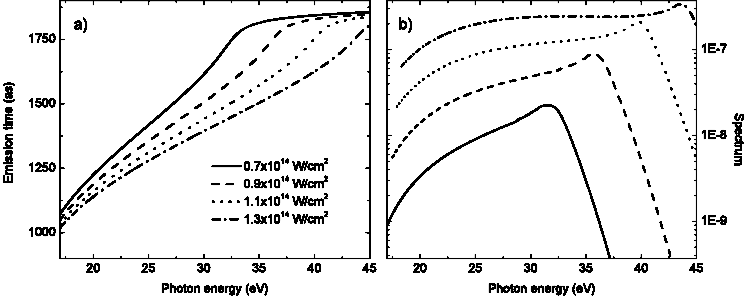
\includegraphics[width=0.8\columnwidth]{Figures/ThreeStep/gdd_argon.pdf}%
\caption{Temps d’émission (gauche) et intensité harmonique (droite) en fonction de l’énergie de photon harmonique et pour différentes intensités de génération. Calcul fait pour l’argon en ne considérant que la trajectoire courte de la GHOE. Tiré de \mycite{DivekiPhD2011}.}
\label{fig:diveki}
\end{figure}

Cette pente linéaire, couramment appelée \textit{atto-chirp}, est donc intrinsèque au mécanisme de génération lui-même \mycite{KazamiasPRA2004}. Elle peut être mesurée expérimentalement, par exemple par la technique RABBIT \mycite{DinuPRL2003,MairesseScience2003}, dont il sera question à la partie \ref{sec:omabbit}. Sa mesure permet également de la compenser, de sorte à comprimer les impulsions attosecondes générées.

\subsection{Phase spatiale des trajectoires quantiques}
\label{sec:phase_spatiale}
Nous avons jusqu'à présent considéré un unique atome émettant un rayonnement harmonique. En réalité, le faisceau de génération a une extension transverse bien plus large qu'un atome, le rayonnement émis est donc la somme cohérente de la contribution de chaque atome unique. Si le faisceau de génération a un profil d'intensité transverse gaussien, son intensité n'est pas uniforme. Nous allons voir que cela se traduit par une phase spatiale non homogène dans l'émission harmonique. On utilise les coordonnées cylindriques $(r,\theta,z)$. En un point $(r,\theta)$ dans le plan transverse, la phase du champ harmonique pour la trajectoire $j$ est donnée par :
\begin{equation}
\phi^j_q = \omega_q t_r - \int_{t_i}^{t_r}\left(\frac{({\bm{p}+\bm{A(t')}})^2}{2}+I_p\right)\rmd t',
\end{equation} 
où $t_i,\;t_r$ et $\bm{p}$ sont les solutions des équations de phase stationnaire. La phase dépend de l'intensité via le potentiel vecteur $\bm{A}(t)$. 

Sur la figure \ref{fig:varju}, tirée de \mycite{VarjuJMO2005}, est tracée $\phi^j_q$ en fonction de l'intensité $I$ pour l'harmonique 19 et pour les deux premières trajectoires quantiques. On observe une dépendance quasiment linéaire, de pente beaucoup plus forte pour la trajectoire longue. Pour les harmoniques loin de l'énergie de coupure, on approxime une dépendance linéaire :
\begin{equation}
\phi^j_q = - \alpha_q^j I,
\label{eq:alphaI}
\end{equation}
où $\alpha_q^j$ est le coefficient de proportionnalité exprimé en $\si{\radian\cm\squared\per\W}$. Cette phase est appelée \textit{phase atomique}. $\alpha_q^{\text{courte}}$ est de l'ordre de $\SI{-1}{\radian\cm\squared\per\W}$ tandis que $\alpha_q^{\text{longue}}\sim\SI{-25}{\radian\cm\squared\per\W}$. Sur le panneau de droite de la figure \ref{fig:varju} est tracé $\partial\phi^j_q/\partial I$ en fonction de l'ordre harmonique. $\alpha_q^{\text{courte}}$ est donc une fonction croissante de l'ordre harmonique, tandis que $\alpha_q^{\text{longue}}$ est décroissante. Dans la coupure, les deux trajectoires se confondent et convergent vers $\approx \SI{-12}{\radian\cm\squared\per\W}$\par
Si on considère maintenant la phase macroscopique du faisceau $\phi^j_q(r,\theta)$ pour une intensité gaussienne, on aura une courbure de phase : la dépendance en intensité du dipôle harmonique modifie la divergence de chaque harmonique. Pour les harmoniques les plus basses, les trajectoires longues auront une divergence bien plus grande que les courtes. Quand l'ordre harmonique augmente, la divergence des trajectoires courtes (resp. longues) augmente (resp. diminue) jusqu'à se confondre à la coupure. Cet effet est bien visible sur les spectres expérimentaux présentés plus loin (figure \ref{Fig:SpectrumGAr}). Il jouera également un rôle central dans la GHOE par un faisceau de Laguerre-Gauss (partie \ref{sec:pmodes}).

\begin{figure}[!ht]
\centering
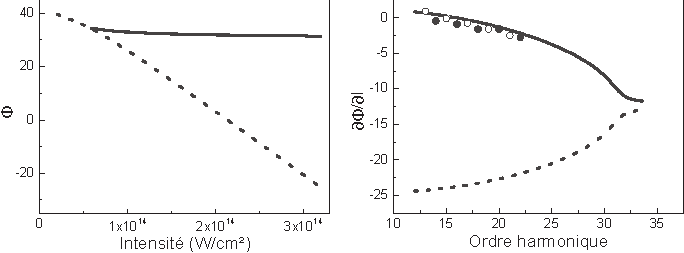
\includegraphics[width=1\columnwidth]{Figures/ThreeStep/alphaI_varju.pdf}%
\caption{Variation de la phase $\phi^j_q$ avec l'intensité (gauche). Le calcul est réalisé pour l'harmonique 19. Variation de $\partial\phi^j_q/\partial I$ avec l'ordre harmonique (droite), à une intensité de $\SI{1.5e15}{\W\per\cm\squared}$. Les lignes continues (resp. pointillées) correspondent aux trajectoires courtes (resp. longues).}
\label{fig:varju}
\end{figure}

\subsection{Accord de phase}
Ces considérations nous amènent à discuter d'un dernier point : l'accord de phase dans la GHOE. Nous avons déjà mentionné que le rayonnement était la somme cohérente de la contribution de chaque atome dans la zone d'interaction. Cette somme doit être réalisé selon la dimension transverse, $(r,\theta)$, et longitudinale, $z$. Si les différentes contributions ne sont pas en phase, des interférences destructives empêcheront l'émission macroscopique de rayonnement XUV. La compréhension de ce phénomène est essentielle pour expliquer les propriétés macroscopiques du rayonnement \mycite{SalieresPRL1995} et pour optimiser le rendement du processus \mycite{KazamiasPRL2003}.

Notons $\bm{k}_q$ le vecteur d'onde de l'harmonique d'ordre $q$ et $\bm{k}_1$ celui du faisceau gaussien de génération. \`A ces deux quantités s'ajoutent des termes de désaccord de phase dus à la phase atomique ainsi qu'à la dispersion électronique et ionique, que l'on note $\Delta \psi_q(r,\theta)$. La condition d'accord de phase pour l'harmonique $q$ s'écrit alors \mycite{BalcouPRA1997} :
\begin{equation}
\bm{k}_q(r,\theta,z) = q\bm{k}_1(r,\theta,z) + \Delta \psi_q(r,\theta,z)
\end{equation}
\mycite{BalcouPRA1997} évaluent le désaccord de phase $|\delta \bm{k}_q| = |\bm{k}_q-q\bm{k}_1 - \Delta \psi_q|$, en négligeant les effets de dispersion sur le laser. La figure \ref{fig:balcou} montre ce désaccord de phase pour les trajectoires courtes et longues. 

\begin{figure}[!ht]
\centering
\includegraphics[width=1\columnwidth]{Figures/ThreeStep/phasematching_balcou.pdf}%
\caption{Désaccord de phase pour les trajectoires longues (gauche) et courtes (droite). Les zones les plus claires indiquent un bon accord de phase. Les pointillés verticaux indiquent les positions des optima de génération d'harmonique. Les flèches représentent la direction d'émission du champ harmonique. Le calcul a été réalisé à une intensité de de \SI{6e14}{\W\per\cm\squared} dans le néon, pour l'harmonique 45. Le paramètre confocal est de 5 mm. Tiré de \mycite{BalcouPRA1997}.}
\label{fig:balcou}
\end{figure}

\'Etudions le cas de la trajectoire longue. On observe une structure particulière, en forme de "moustache de morse". On a deux zones notée B et D où le désaccord de phase est minimisé. La zone notée B est située sur l'axe optique mais est très fine, tandis que la zone D est assez étendue et est située en dehors de l'axe optique. De par le volume disponible, la génération d'harmonique proviendra principalement de la zone D. Les flèches indiquent une émission très divergente, ce qui est dû à l'effet de la phase atomique décrit plus haut. Notons également que la zone D se situe en amont de $z=0$, position du foyer du laser de génération. Pour la trajectoire courte (panneau de droite), le comportement est plus simple : on a un maximum du désaccord de phase vers $z\approx-0.5$ mm, qui diminue ensuite dans toutes les directions. Si on s'éloigne trop du foyer laser, l'intensité devient trop faible pour avoir une génération efficace. \mycite{BalcouPRA1997} montrent que l'optimum se situe à $z=3$ mm, où on a un désaccord faible sur un grand volume. 

En conclusion, nous avons mis en évidence deux familles de trajectoires électroniques, qui donnent lieu à deux composantes dans l'émission harmoniques de propriétés différentes. Finalement, nous avons vu que l'accord de phase permet de favoriser l'une ou l'autre : la trajectoire courte sera accordée lorsque le foyer optique se situe en amont du jet de gaz, tandis que la longue le sera lorsqu'il se situe en aval. Pour une description plus complète de la théorie de la GHOE, on se reportera à \mycite{ScrinziJPB2006} et à \mycite{SmirnovaIvanov2014}. Le modèle SFA présenté ici est la base des calculs numériques présentés plus loin (partie \ref{sec:sfa}), qui prendront en compte tous les effets de propagation et d'accord de phase dans le milieu. Dans la suite de cette partie, nous expliquons comment réaliser une expérience de GHOE dans le cas habituel d'un faisceau de génération gaussien.

\chapter{Aspects expérimentaux de la génération d'harmoniques d'ordre élevé}
\label{Sec:HHG_G}
\section{Système laser}
\label{sec:laser}
Toutes les expériences présentées dans ce chapitre et dans la partie \ref{PA:OAM_HHG} ont été réalisées sur le laser LUCA (Laser Ultra-Court Accordable) du LIDYL au CEA Saclay. Il s'agit d'un laser basé sur la technique "Chirped Pulse Amplification" utilisant le titane saphir comme milieu à gain. Partant d'un oscillateur femtoseconde oscillant autour de 800 nm, le faisceau est étalé temporellement avant d'être amplifié d'abord dans un amplificateur régénératif, puis dans un amplificateur multi-passages. Il est finalement recomprimé dans un compresseur à réseaux \mycite{StricklandOC1985}. La spécificité de ce système est l'insertion récente, juste avant la compression, d'un étage de filtrage modal \mycite{MahieuAPB2015}. Il s'agit d'une fibre creuse de 30 cm de long et $\SI{128}{\micro\metre}$ de diamètre dans laquelle le faisceau est injecté avant d'être collimaté de nouveau. Ceci a pour effet de sélectionner un mode de propagation très proche d'un mode gaussien pur. Finalement on obtient des impulsions dont l'intensité a une enveloppe temporelle gaussienne de largeur à mi-hauteur $\tau = 50$ fs et un profil spatial gaussien de largeur $w_0 = 15$ mm à $\frac{1}{e^2}$. La longueur d'onde utilisée est 792 nm, et l'énergie par impulsion est de 35 mJ pour un taux de répétition de 20 Hz. 

\section{Génération d'harmoniques d'ordre élevé}
Nous commençons par mettre en forme le faisceau laser : son diamètre est ajusté à l'aide d'un iris et son énergie est ajustée grâce à un atténuateur constitué d'une lame demi-onde et d'une paire de polariseur croisés. \`{A} la sortie de cet atténuateur, la polarisation du laser est verticale (S). Le faisceau est ensuite focalisé par une lentille dans un jet de gaz délivré par une vanne pulsée à la fréquence du laser par un système piezo-électrique (Attotech). L'utilisation d'une vanne pulsée permet de n'envoyer du gaz que lorsque le faisceau laser est présent, ce qui limite la pression résiduelle dans les chambres à vide. Ainsi, on peut atteindre une pression assez élevée ($\simeq$10 mbar) dans la région focale sans que l'émission harmonique ne soit réabsorbée par le gaz résiduel. Un autre paramètre important est le diamètre de l'orifice de la vanne (ici, 150 $\si{\micro\metre}$) : en choisissant un diamètre faible, on crée une extension supersonique du gaz ce qui garantit une longueur d'interaction avec le laser courte dans la direction longitudinale. On s'approche ainsi des conditions idéales d'un plan d'atomes, ce qui limite l'importance des effets d'accord de phase dans la GHOE. \par
Le choix du gaz dépend de l'expérience réalisée : on peut par exemple utiliser une molécule dont on étudie la réponse - c'est le principe de la spectroscopie harmonique. Dans notre cas le gaz n'est pas l'objet d'étude et on préférera utiliser un système simple, facile à se procurer, et ayant une grande section efficace. Le gaz le plus courant est l'Argon, qui est peu coûteux et génère de manière très efficace. Son potentiel d'ionisation est de 15.76 eV, ce qui donne une énergie de coupure assez faible et qui empêche de générer des ordres harmoniques très élevés. Dans les cas où on désire générer des ordres élevés et nombreux, on pourra utiliser d'autres gaz rares comme le Néon ($I_p$ = 21.6 eV), bien que la génération soit moins efficace.

Pour notre système, les paramètres nominaux sont :
\begin{itemize}
\item Le diamètre avant focalisation \O{} $\approx$ 10-15 mm,
\item L'énergie par impulsion de l'ordre de E = 1-3 mJ,
\item La lentille de longueur focale f = 1 m. \\
\end{itemize}
Pour connaître la valeur de l'intensité pic au foyer, le profil du faisceau après focalisation peut être calculé numériquement. Le champ avant la lentille est défini dans les coordonnées cylindriques $(R,\theta)$ par :
\begin{equation*}
E(R,\theta) = \sqrt{I_0} \exp{\left(-\frac{R^2}{w_0^2}\right)}\times\delta(\frac{\mbox{\O}}{2}-R),
\end{equation*}
où $w_0$ est la largeur du faisceau collimaté avant l'iris, \O{}  est le diamètre de l'iris, $\delta$ est la fonction de Heaviside, et $I_0 = \frac{2E\sqrt{\frac{4\log{2}}{\pi}}}{\tau\pi w_0^2}$.
La focalisation d'un faisceau par une lentille mince peut être calculée par une transformée de Fourier (voir \mycite{Goodman}, un des ouvrages de référence pour l'optique de Fourier, et \mycite{Tan} pour des exemples d'implémentations numériques). Ces calculs permettent d'étudier l'influence des différents paramètres. Par exemple, on peut faire varier le diamètre de l'iris : la Figure \ref{Fig:IrisScan} montre le profil du faisceau au foyer quand \O{} varie entre 5 et 25 mm. On voit alors que l'intensité pic au foyer part d'une valeur $<10^{13}$ et monte jusqu'à $\SI{10e14}{W/cm²}$. On se trouve donc parfaitement dans le régime d'intensité nécessaire à la génération d'harmonique : l'intensité est suffisante pour enclencher une ionisation tunnel mais reste assez faible pour ne pas ioniser et dépléter tout le milieu.

\begin{figure}[!ht]
\centering
\def\svgwidth{\columnwidth}
\import{Figures/Iris_Scan/}{Fig_IrisScan.pdf_tex}
\caption{\'{E}volution du foyer lorsqu'on varie la taille de l'iris. De gauche à droite : (1) profil transverse de l'intensité au foyer, (2) intensité pic, (3) taille du waist. Les paramètres sont les suivants : E = 1 mJ, $w_0$ = 15 mm, $\tau$ = 50 fs, $\lambda$ = 792 nm, f = 1 m et \O{} variant de 5 à 25 mm par pas de 1 mm. Le calcul est réalisé sur une grille de 1025x1025 points correspondant à une taille réelle de 5*\O{}.}
\label{Fig:IrisScan}
\end{figure}

Les harmoniques d'ordre élevé du laser infrarouge sont ainsi générées par le gaz injecté près du foyer de la lentille. Pour leur détection et caractérisation, nous avons utilisé d'une part un spectromètre électronique à temps de vol, d'autre part un spectromètre de photons. Le premier requiert un rayonnement focalisé alors que le second accepte en entrée un rayonnement divergent. Afin de pouvoir utiliser ces deux diagnostics successivement, avant d'entrer dans le spectromètre, le rayonnement XUV est ré-imagé par un dispositif composé de deux optiques (représentées plus bas sur la figure \ref{Fig:ExpG}) :
\begin{enumerate}
\item Un miroir torique en or de 50 cm de focale. Le miroir travaille à $11.5\degres$ d'incidence rasante ($78.5\degres$ par rapport à la normale au miroir), ce qui permet d'avoir une réflectivité importante et plate sur la gamme spectrale considérée (voir Figure \ref{Fig:TorR}).

\begin{figure}[!ht]
\centering
\def\svgwidth{0.6\columnwidth}
\import{Figures/Reflect_Torique/}{torR.pdf_tex}
\caption{Réflectivité calculée du miroir torique en or à un angle d'incidence de $11.5\degres$. (CXRO, \mycite{Henke1993}).}
\label{Fig:TorR}
\end{figure}
Le miroir torique est utilisé dans une configuration 2f-2f de sorte à garder un rapport\shorthandoff{:} 1:1 \shorthandon{:}entre le foyer de génération et le second foyer. \`{A} la position de ce second foyer nous pouvons placer le spectromètre à temps de vol, qui sert dans le cas d'une mesure RABBIT (voir la partie \ref{sec:omabbit}). Un autre avantage de cette imagerie est d'éloigner la zone de génération, où la pression est élevée, du spectromètre de photons, qui requiert un vide de l'ordre de $10^{-5}$ mbar pour que les détecteurs fonctionnent.\\

\item La deuxième optique est une lame de Si$\mbox{O}_{\mbox{2}}$, qui joue le rôle de filtre de l'infrarouge de génération. La lame de silice est traitée antireflet pour l'infrarouge grâce à un dépôt de multicouches. La dernière de ces couches est en silice, ce qui, combiné à une bonne qualité de surface permet de réfléchir efficacement le rayonnement harmonique. La Figure \ref{Fig:SilR}, tirée de \mycite{MairessePhD}, présente la réflectivité de la lame pour le rayonnement harmonique et infrarouge. La réflectivité dans l'extrême ultra violet (XUV) est donc supérieure à 50\% jusqu'à l'ordre $\approx 37$, tandis que moins de 10\% de l'infrarouge est réfléchi. Le filtrage de l'infrarouge de génération est souvent crucial : il constitue un bruit de mesure non négligeable, sans compter qu'il peut facilement endommager des optiques ou des détecteurs en aval s'il est focalisé.

\begin{figure}[!ht]
\centering
\def\svgwidth{\columnwidth}
\import{Figures/Reflect_Silice/}{silR.pdf_tex}
\caption{Réflectivité de la lame de silice. \`{A} gauche, transmission et réflectivité à 800 nm en fonction de l'angle d'incidence rasante. Les pointillés repèrent notre angle de $11.5\degres$. \`{A} droite, réflectivité XUV mesurée (cercles bleus) et donnée par le CXRO (ligne violette) (\mycite{Henke1993}). Figure adaptée de \mycite{MairessePhD}.}
\label{Fig:SilR}
\end{figure}
\end{enumerate}

Comme nous le verrons plus loin, pour l'étude des faisceaux de Laguerre-Gauss, il sera crucial d'imager le spectre harmonique, c'est-à-dire de séparer les différents ordres harmoniques et de mesurer leurs propriétés spatiales. C'est le rôle du spectromètre de photons. Environ 50 cm en aval du second foyer, les harmoniques sont dispersées par un réseau à pas variable cylindrique Hitachi 001-0437 (voir \mycite{KitaAO1983} pour des détails sur son fonctionnement). Comme pour les réseaux à pas fixe, l'angle de réflexion d'un rayonnement monochromatique de longueur d'onde $\lambda$ est donné par la formule :
\begin{equation*}
m\lambda=\frac{\sin{\alpha}+\sin{\beta}}{\sigma},
\end{equation*}
où $m$ est l'ordre de diffraction considéré (généralement 1), $\sigma$ le nombre de trait par mètre (1200 traits/mm dans notre cas), $\alpha$ et $\beta$ les angles d'incidence et de réflexion, définis par rapport à la normale au réseau (la documentation donne $\alpha = 87$\degres{} pour un fonctionnement optimal).\par
Le réseau de diffraction est cylindrique, le rendant focalisant uniquement dans la dimension horizontale. Un rayonnement gaussien de faible largeur spectrale $\Delta\lambda$ et de largeur spatiale $w(z)$ formera donc dans le plan focal du réseau une fine ligne verticale de largeur proportionnelle à $\Delta\lambda$ et de hauteur $w(z)$. On image ainsi à la fois les dimensions spectrale et spatiale, si on suppose la symétrie cylindrique. Ce spectre est imagé par des galettes de micro-canaux couplées à un écran de phosphore, lui-même observé par une caméra CCD Basler A102f. 

L'intégralité du dispositif expérimental est représenté sur la Figure \ref{Fig:ExpG}.

\vspace{\baselineskip}
\begin{figure}[!ht]
\centering
\def\svgwidth{\columnwidth}
\import{Figures/Setup_G/}{setupG_wbitmap.pdf_tex}
\caption{Dispositif expérimental de génération et détection d'harmoniques d'ordre élevé.}
\label{Fig:ExpG}
\end{figure}

Les figures \ref{Fig:SpectrumGAr} et \ref{Fig:SpectrumGNe} présentent des spectres obtenus avec ce dispositif en utilisant respectivement l'argon et le néon comme gaz de génération. On observe les ordres harmoniques allant de 13 à 29 dans l'argon, et de 13 à 57 dans le néon. Le potentiel d'ionisation du Néon, plus élevé que celui de l'argon, a permis d'utiliser une intensité plus importante sans ioniser complètement le milieu. Conformément à la loi de coupure on obtient dans ce cas un spectre plus étendu. Sur le spectre de l'argon, on observe clairement les deux premières trajectoires quantiques de la GHOE (voir partie \ref{sec:thTraj}) : une contribution sur l'axe correspond à la trajectoire courte et une plus divergente et moins intense correspond à la trajectoire longue. Dans le cas du néon, les conditions d'accord de phase utilisées favorisent la trajectoire courte. On remarque également que la divergence de la trajectoire courte (resp. longue) augmente (rep. diminue) avec l'ordre harmonique, jusqu'à ce que les deux trajectoires se confondent dans la coupure. Notons finalement la présence sur le spectre du néon de pics satellites autour des harmoniques les plus basses : il s'agit des harmoniques plus élevées diffractées au second ordre par le réseau.
\begin{figure}[!ht]
\centering
\def\svgwidth{\columnwidth}
\import{Figures/Spectrum_G/}{Spectrum_G_Ar.pdf_tex}
\caption{Spectre d'harmoniques d'ordre élevé générées dans l'argon à partir d'un mode laser gaussien.}
\label{Fig:SpectrumGAr}
\end{figure}
\begin{figure}[!ht]
\centering
\def\svgwidth{\columnwidth}
\import{Figures/Spectrum_G/}{Spectrum_G_Ne.pdf_tex}
\caption{Spectre d'harmoniques d'ordre élevé générées dans le néon à partir d'un mode laser gaussien.}
\label{Fig:SpectrumGNe}
\end{figure}

\chapter{Le moment angulaire de la lumière}
\label{CH:OAM}

\section{Le moment angulaire en mécanique classique}
\subsection{Le concept de moment angulaire}
\subsubsection{Centre de masse d'un objet}

En mécanique classique, l'évolution d'un objet est décrit par les lois de Newton. Pour un objet ''ponctuel'', on a ainsi $\sum_i{\bm{F_i}}=m\bm{a}$, où $\bm{F_i}$ sont les forces appliquées à cet objet, $m$ sa masse et $\bm{a}$ son accélération. Si on s'intéresse maintenant à un objet plus complexe, tel qu'un atome, un fluide ou une galaxie, il faut prendre en compte l'effet de la structure interne de l'objet : un objet réel peut se déformer de multiples façons sous l'effet des forces reliant les éléments qui le constituent.

Considérons donc un objet non ponctuel. Si on lance un tel objet en l'air, son comportement sera plus compliqué qu'une particule ponctuelle : notre objet peut tourner, vaciller, se déformer, etc. On peut quand même considérer notre objet comme constitué de nombreuses particules, reliées entre elles par de diverses forces. On sait alors que la force appliquée sur l'objet \textit{i} est sa masse fois son accélération : $\bm{F_i} = d^2(m_i\bm{r_i})/dt^2$. \\La trajectoire de notre objet ressemble toutefois à une parabole, même si ce n'est pas le cas pour chacune des particules qui le constituent. Ce quelque chose qui décrit une parabole est le \textit{centre de masse} de l'objet. Si on note $M$ la masse totale du système, il est définit par le vecteur $\bm{R}$ :
\begin{equation*}
\bm{R} = \sum_i{m_i\bm{r_i}/M}.
\end{equation*}
La trajectoire de ce point inventé artificiellement est facile à décrire en utilisant le \textit{théorème du centre de masse}, qui nous dit que la somme des forces appliquées à toutes les particules constituant l'objet est égale à :
\begin{equation*}
\bm{F} = \sum_i{\bm{F_i}} = \frac{d^2(\sum_i{m_i\bm{r_i}})}{dt^2} = \frac{d^2(M\bm{R})}{dt^2} = \frac{Md^2(\bm{R})}{dt^2}.
\end{equation*}
Remarquons ici que $\bm{F}$, la somme des forces appliquées à toutes les particules, est égale aux forces \textit{extérieures} au système. En effet, quelque soit la nature des forces internes à notre objet, ces forces s'exercent entre deux particules et la troisième loi de Newton nous dit qu'entre ces particules l'action égale toujours la réaction. Ainsi dans le terme $\sum_i{\bm{F_i}}$, les forces internes s'annulent deux à deux pour l'objet considéré.\\ Cette propriété du centre de masse est particulièrement importante et est d'ailleurs la raison pour laquelle nous l'avons introduit : nous voyons que les mécaniques \textit{internes} et \textit{externes} de l'objet peuvent être traitées séparément. Ainsi, nous allons pouvoir nous concentrer sur les mouvements internes de notre objet, et en particulier sa rotation.

\subsubsection{Rotation d'un corps rigide}
Comme nous l'avons noté plus haut, le comportement d'un objet réel est plus complexe qu'une simple rotation. Pour simplifier cette discussion nous allons considérer un objet rigide, c'est-à-dire constitué d'un certain nombres de particules reliées par des forces assez fortes pour que l'objet ne se déforme pas au cours du mouvement. Nous considérons également le problème à deux dimensions seulement, et généraliserons ensuite le résultat.

Si nous ignorons le mouvement du centre de masse, la seule chose que peut faire notre objet est tourner autour d'un axe. Cet axe est défini comme l'endroit de l'objet restant au repos. La rotation autour de cet axe est alors simplement définie par l'évolution de l'angle d'un quelconque point de l'objet au cours du temps. On peut décrire la rotation à deux dimensions de la même façon qu'une translation à une dimension : l'angle $\theta$ est l'analogue de la distance de laquelle s'est déplacé l'objet, et la vitesse angulaire $\omega=d\theta/dt$ est l'analogue de la vitesse à laquelle se déplace l'objet. Notons maintenant $(x,y)$ les coordonnées cartésiennes de notre espace à deux dimensions. Si l'angle de l'objet a changé d'une petite quantité $\Delta\theta$ après un temps $\Delta t$, alors les changements selon $x$ et $y$ sont simplement :
\begin{equation*}
\Delta x = -y\Delta \theta \mbox{ et } \Delta y = x\Delta \theta
\end{equation*}
On peut maintenant chercher à définir ce qui ''crée'' cette rotation. De la même manière qu'un mouvement linéaire est créé par une force, une rotation est créée par quelque chose appelé le \textit{couple}. Une force peut être définie par son \textit{travail} lors d'un déplacement $\Delta x$ de son point d'application. Par analogie, le couple peut être défini par son travail lors d'une rotation $\Delta \theta$. Lors d'une rotation d'angle très faible, le travail fournit est 
\begin{equation*}
\Delta W = F_x \Delta x + F_y \Delta y.
\end{equation*}
En substituant directement $\Delta x$ et $\Delta y$, on obtient
\begin{equation*}
\Delta W = (xF_y-yF_x)\Delta \theta,
\end{equation*}
Ce qui nous fournit l'expression du couple en fonction de la force appliquée :
\begin{equation*}
\tau = (xF_y-yF_x).
\end{equation*}

\subsubsection{Moment angulaire}
Cette analogie nous amène à définir une dernière quantité. Pour une translation linéaire, on sait que la force externe au système est égale à $d(m\bm{r})/dt$, c'est à dire au taux de variation d'une quantité $\bm{p}$ appelée moment total de l'objet. De même, le couple appliqué au système est égal au taux de variation de $L$, appelé \textit{moment angulaire} de l'objet. On peut effectivement écrire :
\begin{equation}
\tau = xF_y-yF_x = xm(d^2y/dt^2)-ym(d^2x/dt^2) = \frac{d}{dt}\biggl[xm\biggl(\frac{dy}{dt}\biggr) - ym\biggl(\frac{dx}{dt}\biggr)\biggr].
\label{Eq.DefTauL}
\end{equation}
$\tau$ est donc bien égal à la variation temporelle d'une quantité dont on obtient l'expression :
\begin{equation*}
L = xm\biggl(\frac{dy}{dt}\biggr) - ym\biggl(\frac{dx}{dt}\biggr) = xp_y - yp_x.
\end{equation*}
Nous avons jusqu'à présent considéré un problème à deux dimensions par simplicité. Si l'on considère maintenant un espace à trois dimensions $(x,y,z)$, les résultats obtenus sont valables pour une rotation dans le plan $xy$, c'est à dire autour de l'axe $z$. On définit donc $L_z$, le moment angulaire selon l'axe $z$. Nous pouvons le faire pour n'importe quel axe, et obtenir pour les trois axes de notre repère
\begin{equation}
\begin{alignedat}{6}
&L_x~&&=y&&p_z&&-z&&p_y&&,\\
&L_y~&&=z&&p_x&&-x&&p_z&&,\\
&L_z~&&=x&&p_y&&-y&&p_x&&.
\end{alignedat}
\label{Eq.Ldef}
\end{equation}
Le moment angulaire à trois dimensions est donc un vecteur, dont les composantes sont données par Eq. \ref{Eq.Ldef}. Il est pratique de réécrire cette expression sous forme vectorielle :
\begin{equation*}
\bm{L}=\bm{r}\times\bm{p}
\end{equation*}
Pour terminer, regardons à nouveau l'expression \ref{Eq.DefTauL} : la variation de $\bm{L}$ est égale au couple total appliqué au système. Comme expliqué plus haut, $\bm{F_{tot}} = \bm{F_{ext}}$. En utilisant de la même manière la troisième loi de Newton, on obtient que 
\begin{equation*}
\bm{\tau_{tot}} = \bm{\tau_{ext}} = \frac{d\bm{L}}{dt}. 
\end{equation*}
Ce résultat est très important puisqu'il nous donne \textit{la loi de conservation du moment angulaire} : si aucun couple extérieur n'est appliqué à un système de particules, alors son moment angulaire reste constant.


\subsection{Le cas de la lumière}
\subsubsection{L'énergie du champ électromagnétique}
La partie précédente s'intéressait au moment angulaire porté par la matière. Cette matière est également capable d'émettre des radiations lumineuses, et en se faisant peut perdre de l'énergie. Pour respecter la conservation de l'énergie, il est donc nécessaire que la lumière, et plus généralement les ondes électromagnétiques, portent de l'énergie.

Considérons une distribution de charges et de courants contenus dans un volume $V$. En un court temps $dt$, une charge bougera de $\bm{v}dt$ et en utilisant l'expression de la force de Lorentz, le travail effectué sur la charge sera
\begin{equation*}
dU = \bm{F}\cdot\bm{dl} = q(\bm{E}+\bm{v}\times\bm{B})\cdot\bm{v}dt = q\bm{E}\cdot \bm{v} dt,
\end{equation*}
où l'on retrouve que la force magnétique ne fournit pas de travail. Notons ensuite $q = \rho dV$ la densité de charge dans le volume et $\rho \bm{v} = \bm{J}$ la densité de courant. En intégrant sur le volume V, on obtient
\begin{equation*}
\frac{dU}{dt} = \int_V \bm{E} \cdot \bm{J} dV.
\end{equation*}
$dU/dt$ est le taux auquel le travail est fournit, c'est-à-dire la puissance délivrée au système. $\bm{E} \cdot \bm{J}$ est donc la puissance délivrée par une unité de volume, que l'on peut exprimer en utilisant l'équation de Maxwell-Ampère :
\begin{align*}
\bm{E} \cdot \bm{J} &= \frac{1}{\mu_0}\bm{E} \cdot (\bm{\nabla} \times \bm{B})-\epsilon_0\bm{E}\cdot\frac{\partial\bm{E}}{\partial t}\\
&= \frac{1}{\mu_0}\bigl[\bm{B} \cdot (\bm{\nabla} \times \bm{E})-\bm{\nabla} \cdot (\bm{E} \times \bm{B})\bigr]-\epsilon_0\bm{E}\cdot\frac{\partial\bm{E}}{\partial t}\\
&= \frac{1}{\mu_0}\bigl[-\bm{B} \cdot \frac{\partial\bm{B}}{\partial t}-\bm{\nabla} \cdot (\bm{E} \times \bm{B})\bigr]-\epsilon_0\bm{E}\cdot\frac{\partial\bm{E}}{\partial t}
\end{align*}
On note que $\bm{B} \cdot \frac{\partial\bm{B}}{\partial t} = \frac{1}{2}\frac{\partial\bm{B^2}}{\partial t}$ et $\bm{E} \cdot \frac{\partial\bm{E}}{\partial t} = \frac{1}{2}\frac{\partial\bm{E^2}}{\partial t}$ et on obtient
\begin{equation*}
\bm{E} \cdot \bm{J} = -\frac{1}{2}\frac{\partial}{\partial t}\biggl(\epsilon_0\bm{E^2}+\frac{1}{\mu_0}\bm{B^2}\biggl)-\frac{1}{\mu_0}\bm{\nabla} \cdot (\bm{E} \times \bm{B})
\end{equation*}
On intègre ensuite cette équation sur le volume $V$ et on utilise le théorème d'Ostrogradski sur le dernier terme pour obtenir
\begin{equation*}
\frac{dU}{dt} = -\frac{\partial}{\partial t}\int_V\frac{1}{2}\biggl(\epsilon_0\bm{E^2}+\frac{1}{\mu_0}\bm{B^2}\biggl)dV-\frac{1}{\mu_0} \oint_S(\bm{E} \times \bm{B})\cdot\bm{dS}
\end{equation*}
Regardons les termes obtenus dans cette expression :
\begin{itemize}
\item Le terme de gauche est la puissance délivrée au volume, soit le taux auquel les particules \textit{gagnent} de l'énergie,
\item Le premier terme de droite est le taux de \textit{pertes} d'énergie électromagnétique dans le champ à \textit{l'intérieur} du volume,
\item Le deuxième terme de droite est le taux de transport de l'énergie \textit{en dehors} du volume, i.e. à travers la surface $S$,
\end{itemize}
On peut donc l'exprimer par:\\\'Energie \textit{perdue} par le champ = énergie \textit{gagnée} par les particules + flux d'énergie en dehors du volume. On peut directement identifier le vecteur :
\begin{equation*}
\bm{S} = \frac{1}{\mu_0}\bm{E}\times\bm{B}
\end{equation*}
comme la \textbf{densité de flux d'énergie} (énergie par unité de surface par unité de temps), connu sous le nom de \textbf{vecteur de Poynting}, d'après John H. Poynting qui a dérivé son expression en 1884 \mycite{Poynting1884}. 
%\chapter{Le moment angulaire orbital dans la génération d'harmoniques d'ordre élevé}
\label{CH:OAM_HHG}
%
\section{Revue des utilisations pratiques des modes de Laguerre-Gauss}
\subsection{Le domaine visible et infrarouge}
\subsection{De plus courtes longueurs d'ondes : perspectives d'applications dans l'extrême ultra-violet}
\subsection{Des durées ultra-brèves : utilisations possibles d'impulsions attosecondes portant du moment angulaire orbital}

\section{Génération d'harmoniques d'ordre élevé à partir de modes de Laguerre-Gauss}

Ayant passé en revue les utilisations envisagées de faisceaux de Laguerre-Gauss de durées ultra-brève et dans le domaine de l'extrême ultra-violet (XUV), nous décrirons ici comment les générer de manière expérimentale. Nous commencerons par détailler notre dispositif de génération d'harmoniques d'ordre élevé dans le cas habituel d'un mode laser Gaussien, puis expliquerons comment passer au cas Laguerre-Gaussien avant de donner les résultats obtenus.

\subsection{Le cas Gaussien : Aspects expérimentaux de la génération d'harmoniques d'ordre élevé}
\label{Sec:HHG_G}
\subsubsection{Système laser}
Toutes les expériences présentées dans ce chapitre ont été réalisées sur le laser LUCA (Laser Ultra-Court Accordable) du LIDYL au CEA Saclay. Il délivre des impulsions ayant une enveloppe temporelle gaussienne de largeur à mi-hauteur $\tau = 50$ fs et une enveloppe spatiale gaussien de largeur à mi-hauteur $w_0 = 15$ mm à $\frac{1}{e^2}$. La longueur d'onde utilisée est 800 nm, et le taux de répétition est de 20 Hz. Ce système dispose d'une fibre utilisée pour filtrer spatialement le faisceau, ce qui garantit un profil très proche d'un mode gaussien pur \mycite{MahieuAPB2015}. Le prix à payer est une diminution de l'énergie par impulsion, qui atteint quand même environ 35 mJ après la fibre et le dernier étage de compression.

\subsubsection{Génération d'harmoniques d'ordre élevé}
Nous commençons par mettre en forme le faisceau laser : son diamètre est ajusté à l'aide d'un iris et son énergie est ajustée grâce à un atténuateur constitué d'une lame demi-onde et d'une paire de polariseur croisés. \`{A} la sortie de cet atténuateur, la polarisation du laser est verticale (S). Le faisceau est ensuite focalisé par une lentille dans un jet de gaz délivré par une vanne pulsée à la fréquence du laser par un système piezo-électrique (Attotech). L'utilisation d'une vanne pulsée permet de n'envoyer du gaz que lorsque le faisceau laser est présent, ce qui limite la pression résiduelle dans les chambres à vide. Ainsi, on peut atteindre une pression assez élevé (XXX) dans la région focale sans que l'émission harmonique ne soit réabsorbée par le gaz résiduel. Un autre paramètre important est le diamètre de l'orifice de la vanne (ici, 150 $\mu m$) : en choisissant un diamètre faible, on crée une extension supersonique du gaz ce qui garantit une longueur d'interaction faible avec le laser. On s'approche ainsi des conditions idéales d'un plan d'atomes, ce qui limite l'importance des effets d'accord de phase dans la GHOE. \par
Le choix du gaz dépend de l'expérience réalisée : on peut par exemple utiliser une molécule dont on étudie la réponse, on parle alors de spectroscopie harmonique. Le gaz n'est pas l'objet d'étude dans notre cas, on préférera donc choisir un système simple, facile à se procurer, et ayant une grande section efficace. Le gaz le plus courant est l'Argon, qui est peu coûteux et génère de manière très efficace. Son potentiel d'ionisation est de 15.76 eV, ce qui donne une énergie de coupure assez faible et qui empêche de générer des ordres harmoniques très élevés. Dans les cas où on désire générer des ordres élevés et nombreux, on pourra utiliser d'autres gaz rares comme le Néon ($I_p$ = 21.6 eV) même si la génération sera moins efficace.

Pour notre système, les paramètres nominaux sont :
\begin{itemize}
\item Le diamètre avant focalisation \O{} $\approx$ 10-15 mm,
\item L'énergie par impulsion de l'ordre de E = 1 mJ,
\item La lentille de longueur focale f = 1 m. \\
\end{itemize}
Pour calculer la valeur de l'intensité pic au foyer, on peut calculer le profil du faisceau après focalisation, par exemple par un calcul numérique. Le champ avant la lentille est défini dans les coordonnées cylindriques $(R,\theta)$ par :
\begin{equation*}
E(R,\theta) = \sqrt{I_0} \exp{\left(-\frac{R^2}{w_0^2}\right)}\times\delta(\frac{\mbox{\O}}{2}-R),
\end{equation*}
où $w_0$ est la largeur du faisceau collimaté avant l'iris, \O{}  est le diamètre de l'iris, $\delta$ est la fonction de Heaviside, et $I_0 = \frac{2E\sqrt{\frac{4\log{2}}{\pi}}}{\tau\pi w_0^2}$.
La focalisation d'un faisceau par une lentille mince peut être calculée par une transformée de Fourier (voir \mycite{Goodman}, un des ouvrages de référence pour l'optique de Fourier, et \mycite{Tan} pour des exemples d'implémentations numériques). Il est alors simple de voir l'effet des différents paramètres expérimentaux. Par exemple, on peut faire varier le diamètre de l'iris : la Figure \ref{Fig:IrisScan} montre le profil du faisceau au foyer quand \O{} varie entre 5 et 25 mm. On voit alors que l'intensité pic au foyer évolue entre 0 et 10 $\times 10^{14} \mbox{W/cm}^2$. On se trouve donc parfaitement dans le régime d'intensité nécessaire à la génération d'harmonique : l'intensité est suffisante pour enclencher une ionisation tunnel mais reste assez faible pour ne pas ioniser et dépléter tout le milieu.

\begin{figure}[!ht]
\centering
\def\svgwidth{\columnwidth}
\import{Figures/Iris_Scan/}{Fig_IrisScan.pdf_tex}
\caption{\'{E}volution du foyer lorsqu'on varie la taille de l'iris. De gauche à droite : (1) profil transverse de l'intensité au foyer, (2) intensité pic, (3) taille du waist. Les paramètres sont les suivants : E = 1 mJ, $w_0$ = 15 mm, $\tau$ = 50 fs, $\lambda$ = 792 nm, f = 1 m et \O{} variant de 5 à 25 mm par pas de 1 mm. Le calcul est réalisé sur une grille de 1025x1025 points correspondant à une taille réelle de 5*\O{}.}
\label{Fig:IrisScan}
\end{figure}

Les harmoniques d'ordre élevé du laser infrarouge sont ainsi générées par le gaz situé près du foyer de la lentille. Ce rayonnement XUV est ensuite ré-imagé par un dispositif composé de deux optiques :
\begin{enumerate}
\item Un miroir torique en or de 50 cm de focale. Le miroir travaille à $11.5\degres$ d'incidence rasante ($78.5\degres$ si on défini l'angle par rapport à la normale au miroir), ce qui permet d'avoir une réflectivité importante et plate sur la gamme spectrale considérée (voir Figure \ref{Fig:TorR}).

\begin{figure}[!ht]
\centering
\def\svgwidth{0.6\columnwidth}
\import{Figures/Reflect_Torique/}{torR.pdf_tex}
\caption{Réflectivité calculée du miroir torique en or à un angle d'incidence de $11.5\degres$. (CXRO, \mycite{Henke1993}).}
\label{Fig:TorR}
\end{figure}

Le miroir toroïdal est positionné dans une configuration 2f-2f de sorte à garder un rapport 1:1 entre le foyer de génération et le second foyer. Ré-imager le foyer de génération est utile car on peut focaliser le rayonnement harmonique dans un deuxième dispositif, comme par exemple un spectromètre à temps de vol dans le cas d'une mesure RABBIT (voir ChapitreXX et YY). Un autre avantage est qu'il éloigne la zone de génération, où la pression est élevée, de la zone de détection, qui requiert souvent un vide de qualité pour que les détecteurs fonctionnent.\\

\item La deuxième optique est une lame de Si$\mbox{O}_{\mbox{2}}$, qui réalise le rôle de filtrage de l'infrarouge de génération. La lame de silice est traitée antireflet pour l'infrarouge grâce à un dépôt de multicouches. La dernière de ces couches est en silice, ce qui combiné à une bonne qualité de surface permet de réfléchir efficacement le rayonnement harmonique. La Figure \ref{Fig:SilR}, tirée de \mycite{MairessePhD} présente la réflectivité de la lame pour le rayonnement harmonique et infrarouge. La réflectivité dans l'XUV est donc supérieure à 50\% jusqu'à l'ordre $\approx 37$, tandis que moins de 10\% de l'infrarouge est réfléchi. Le filtrage de l'infrarouge de génération est souvent crucial : il constitue un bruit de mesure non négligeable, sans compter qu'il peut facilement endommager des optiques ou des détecteurs en aval s'il est focalisé.

\begin{figure}[!ht]
\centering
\def\svgwidth{\columnwidth}
\import{Figures/Reflect_Silice/}{silR.pdf_tex}
\caption{Réflectivité de la lame de silice. \`{A} gauche, transmission et réflectivité à 800 nm en fonction de l'angle d'incidence rasante. Les pointillés repèrent notre angle de $11.5\degres$. \`{A} droite, réflectivité XUV mesurée (cercles) et donnée par le CXRO (lignes) (\mycite{Henke1993}). Figure adaptée de \mycite{MairessePhD}.}
\label{Fig:SilR}
\end{figure}
\end{enumerate}

Nous souhaiterions ensuite pouvoir imager le spectre harmonique, c'est-à-dire séparer les différents ordres harmoniques et mesurer leurs propriétés spatiales. Un peu après le second foyer, les harmoniques sont dispersées par un réseau à pas variable Hitachi 001-0437 (voir \mycite{KitaAO1983} pour des détails sur son fonctionnement). L'angle de réflexion d'un rayonnement monochromatique de longueur d'onde $\lambda$ est donné par la formule des réseau :
\begin{equation*}
m\lambda=\frac{\sin{\alpha}+\sin{\beta}}{\sigma},
\end{equation*}
où $m$ est l'ordre de diffraction considéré (généralement 1), $\sigma$ le nombre de trait par mètre (1200 traits/mm dans notre cas), $\alpha$ et $\beta$ les angles d'incidence et de réflexion, définis par rapport à la normale au réseau (la documentation donne $\alpha = 87$\degres{} pour un fonctionnement optimal).\par
Le réseau de diffraction est cylindrique : il est focalisant dans la dimension horizontale mais est plan dans la direction verticale. Un rayonnement gaussien de faible largeur spectrale $\Delta\lambda$ et de largeur spatiale $w(z)$ formera donc dans le plan focal du réseau une fine ligne verticale de largeur proportionnelle à $\Delta\lambda$ et de hauteur $w(z)$. On image ainsi à la fois les dimensions spectrale et spatiale, si on suppose la symétrie cylindrique. Ce spectre est imagé par des galettes de micro-canaux couplées à un écran de phosphore, lui-même observé par une caméra CCD Basler A102f. 

L'intégralité du dispositif expérimental est représenté sur la Figure \ref{Fig:ExpG}.
\newpage
\vspace{\baselineskip}
\begin{figure}[!ht]
\centering
\def\svgwidth{\columnwidth}
\import{Figures/Setup_G/}{setupG_wbitmap.pdf_tex}
\caption{Dispositif expérimental de génération et détection d'harmoniques d'ordre élevé.}
\label{Fig:ExpG}
\end{figure}

Les figures \ref{Fig:SpectrumGAr} et \ref{Fig:SpectrumGNe} présentent des spectres obtenus avec ce dispositif en utilisant respectivement l'argon et le néon comme gaz de génération. On observe les ordres harmoniques allant de 13 à 29 dans l'argon, et de 13 à 57 dans le néon, la différence d'énergie de coupure étant attendue puisque le néon a un $I_p$ plus élevé. Sur le spectre de l'argon, on observe clairement les deux trajectoires quantiques de la GHOE : une contribution sur l'axe correspond à la trajectoire courte et une plus divergente et moins intense correspond à la trajectoire longue. Dans le cas du néon, les conditions d'accord de phase utilisées favorisent la trajectoire courte. On remarque également que la divergence de la trajectoire courte (resp. longue) augmente (rep. diminue) avec l'ordre harmonique, jusqu'à ce que les deux trajectoires se confondent dans la coupure. Notons finalement la présence sur le spectre du néon de pics satellites autour des harmoniques les plus basses : il s'agit des harmoniques plus élevées diffractées au second ordre par le réseau.
\begin{figure}[!ht]
\centering
\def\svgwidth{\columnwidth}
\import{Figures/Spectrum_G/}{Spectrum_G_Ar.pdf_tex}
\caption{Spectre d'harmoniques d'ordre élevé générées dans l'argon à partir d'un mode laser gaussien.}
\label{Fig:SpectrumGAr}
\end{figure}
\begin{figure}[!ht]
\centering
\def\svgwidth{\columnwidth}
\import{Figures/Spectrum_G/}{Spectrum_G_Ne.pdf_tex}
\caption{Spectre d'harmoniques d'ordre élevé générées dans le néon à partir d'un mode laser gaussien.}
\label{Fig:SpectrumGNe}
\end{figure}

\subsection{Génération de modes de Laguerre-Gauss dans le visible et proche infrarouge}
Ayant décrit la génération ``habituelle'' d'harmoniques d'ordre élevé, décrivons maintenant l'expérience où le laser générateur possède un mode de Laguerre-Gauss, dont l'expression a été donnée au chapitre précédent (équation \ref{eq:lgmodes}). Les modes de Laguerre-Gauss possèdent un moment angulaire orbital bien défini grâce à leur phase hélicoïdale. Plus précisément, c'est le terme $e^{\rmi\ell\theta}$, également présent dans les modes de Bessel, qui leur confère cette propriété. Il sera question de l'index radial $p$ des modes de Laguerre-Gauss plus loin dans cette thèse, mais il n'a pour l'instant pas d'importance pour notre problème. La première question est donc de savoir comment produire un mode de Laguerre-Gauss d'index $(\ell_{IR},0)$ dans l'infrarouge. 

\subsubsection{Superposition de modes de Hermite-Gauss}
\label{sec:hg_modes}
Les faisceaux de LG étant des modes du champ électromagnétique, on peut d'abord penser à modifier le laser lui-même pour qu'il lase directement dans le mode désiré. En introduisant des éléments absorbants dans la cavité, il est a priori possible d'interdire la génération d'un mode Gaussien. En pratique, il est assez compliqué de sélectionner un mode de LG. Il est par contre assez simple de sélectionner un des modes de \textit{Hermite-Gauss}, qui sont les solutions de l'équation d'onde en coordonnées cartésiennes. Ces modes sont souvent appelés modes $\mbox{TEM}_{nm}$, pour ``Transverse Electro-Magnetic'', dont le mode Gaussien $\mbox{TEM}_{00}$ n'est simplement que le mode d'index le plus bas. Quelques uns de ces modes sont représentés sur la figure \ref{Fig:hgmodes}. En insérant simplement un fil vertical (resp. horizontal) dans la cavité laser, on bloque la génération du $\mbox{TEM}_{00}$ et on obtient un mode $\mbox{TEM}_{01}$ (resp. $\mbox{TEM}_{10}$).

\begin{figure}[!ht]
\centering
\def\svgwidth{\columnwidth}
\import{Figures/Mode_Converter/}{HG_Modes.pdf_tex}
\caption{Modes de Hermite-Gauss pour différentes valeurs de $(n,m)$. De gauche à droite, $(n,m) =$ (0,0), (1,0), (0,1), (2,0), (2,1), (3,3). Le code couleur est le même que celui de la figure \ref{Fig:LGModes} : la couleur donne la phase et la luminosité l'intensité.}
\label{Fig:hgmodes}
\end{figure}

Les faisceaux de Hermite-Gauss constituent également une base des modes du champ, dans laquelle on peut donc écrire les modes de Laguerre-Gauss. On peut montrer (\mycite{BeijersbergenOC1993}) que les composantes du mode $\mathcal{LG}_{\ell,p}$ sont égales aux composantes d'un mode $\mbox{TEM}_{nm}$ incliné à 45\degres{} avec $p = \mathrm{min}(m,n)$ et $\ell=m-n$, la seule différence étant l'ajout d'une phase de $\pi/2$ entre les différentes composantes successives. Par exemple pour $\ell = 1$,
\begin{align*}
\mbox{TEM}_{n,m}^{45\mbox{\degres}}&=\frac{1}{\sqrt{2}}\mbox{TEM}_{01}+\frac{1}{\sqrt{2}}\mbox{TEM}_{10} \mbox{ et}\\
\mathcal{LG}_{1,0}&=\frac{1}{\sqrt{2}}\mbox{TEM}_{01}+\frac{\rmi}{\sqrt{2}}\mbox{TEM}_{10}.
\end{align*}
Pour $\ell = 2$, 
\begin{equation*}
\mathcal{LG}_{2,0}=\frac{1}{2}\mbox{TEM}_{02}+\frac{\rmi}{\sqrt{2}}\mbox{TEM}_{11}-\frac{1}{\sqrt{2}}\mbox{TEM}_{20}
\end{equation*}
et ainsi de suite.
Comme dit plus haut, il est possible de générer un mode $\mbox{TEM}_{n,m}$ en cavité, il reste seulement à l'incliner à 45\degres par rapport au repère choisi. Pour contrôler la phase entre les composantes relatives, les auteurs de \mycite{BeijersbergenOC1993} ont montré qu'on pouvait utiliser des lentilles cylindriques. En effet, une lentille cylindrique convergente ne focalise qu'une seule des composantes cartésiennes, qui va subir un déphasage au passage du foyer dû à la phase de Gouy. On recollimate ensuite le faisceau avec une deuxième lentille cylindrique de même focale $f$. La phase ajoutée est ajustée en changeant la distance entre ces deux lentilles; pour obtenir $\pi/2$ il faut choisir $\sqrt{2}f$. La Figure \ref{Fig:Modeconv} illustre le principe de ce dispositif, appelé convertisseur de mode.

\begin{figure}[!ht]
\centering
\def\svgwidth{0.5\columnwidth}
\import{Figures/Mode_Converter/}{mode_converter.pdf_tex}
\caption{Schéma de fonctionnement d'un convertisseur de mode : en partant d'un $\mbox{TEM}_{01}$ incliné à 45\degres, on obtient un mode $\mathcal{LG}_{1,0}$. Tiré de \mycite{PadgettAllen1999}.}
\label{Fig:Modeconv}
\end{figure}

L'intérêt de ce dispositif est de créer des modes purs : on obtient exactement le faisceau de Laguerre-Gauss recherché. Il présente cependant deux inconvénients : (1) il faut disposer d'un mode $\mbox{TEM}_{0\ell}$ au départ, ce qui devient compliqué dès que $\ell$ augmente. De plus, il est peu pratique de devoir modifier la cavité laser, particulièrement dans le cas des lasers de puissances utilisés pour la HHG. (2) Le faisceau est focalisé dans une dimension entre les deux lentilles. La puissance fournie par notre laser imposerait de réaliser la conversion dans une enceinte à vide, sans quoi la focalisation dans l'air détruira le profil spatial et temporel du faisceau. Pour ces raisons, nous avons choisi une méthode plus flexible et plus adapté à un laser de puissance.

\subsubsection{Utilisation d'une lame de phase à spirale}
Cette technique est probablement la façon la plus intuitive d'ajouter le terme de phase qui nous intéresse au faisceau. Pour rajouter une phase $e^{\rmi\ell\theta}$, il suffit d'utiliser une lame de verre transparente dont l'épaisseur varie proportionnellement à $\theta$. On forme ainsi une \textit{lame de phase à spirale} (Spiral Phase Plate, SPP), concept proposé dans \mycite{BeijersbergenOC1994} et représenté sur la Figure \ref{Fig:SPP}.\par
\begin{figure}[!ht]
\centering
\def\svgwidth{0.5\columnwidth}
\import{Figures/SPP/}{SPP.pdf_tex}
\caption{Lame de phase à spirale. La flèche rouge représente le trajet d'un rayon optique. Adapté de \mycite{YaoAOP2011}.}
\label{Fig:SPP}
\end{figure}
La lame présente une discontinuité pour $\theta=0$\degres, dont la hauteur h permet de contrôler le moment angulaire orbital transféré au faisceau pour une longueur d'onde donnée. Si cette hauteur est assez faible pour que l'on reste dans le régime paraxial, on peut considérer que la lame agit uniquement sur la phase du faisceau incident. Ainsi si on choisit 
\begin{equation*}
h = \frac{\ell\lambda}{n-1},
\end{equation*}
où $n$ est l'indice de réfraction du milieu, pour un champ d'entrée $u(r,\theta,z)$ on obtient directement après la lame $u' = u\exp{(-\rmi \ell \theta)}$.	Il est donc non seulement possible de passer d'un mode Gaussien à un mode Laguerre-Gaussien, mais encore de changer l'indice d'un mode déjà Laguerre-Gaussien.\par
La lame de phase illustre joliment la création de MAO : si on considère une onde plane arrivant perpendiculairement à la surface plane de la lame, le rayon qui sort de la lame sera dévié par réfraction à travers la surface hélicoïdale. Cette réfraction se fait dans la direction azimutale, le moment linéaire de la lumière acquière donc une composante azimutale, synonyme de moment angulaire. Plus précisément, pour un rayon $r$ donné, l'angle de la surface	vaut $h/(2\pi r)$. Si on applique la loi de Snell-Descartes on obtient que le rayon est dévié d'un angle $\alpha = (n-1)\ell\lambda/(2\pi r(n-1)) = \ell/(k_0r)$. Le moment linéaire par photon vaut $\hbar k_0$, donc le moment angulaire par photon vaut $r\times\hbar k_0\times\ell/(k_0r) = \ell\hbar$.


Si le principe d'une SPP est simple, sa construction est beaucoup plus compliquée. Les tolérances sur la valeur de h et la régularité de la surface sont très strictes aux longueurs d'ondes optiques, sans quoi la qualité du mode de sortie sera détériorée (si h n'est pas adapté, on peut même créer des modes d'indice non entier, cf. \mycite{LeachNJP2004}). D'ailleurs, lors des premiers travaux sur le sujet (\mycite{BeijersbergenOC1994}), la température de la lame était ajustée pour accorder précisément la hauteur de la lame à la longueur d'onde. La technique a évolué et il est maintenant possible de créer des SPP de très bonne qualité \mycite{OemrawsinghAO2004}.

Enfin, remarquons que même pour une SPP parfaite, la conversion d'un mode à l'autre n'est jamais idéale. La SPP agit sur la phase du faisceau, mais ne modifie pas le profil d'intensité. Ainsi, à sa sortie le champ électrique a la bonne phase mais pas la distribution d'intensité d'un mode de Laguerre-Gauss (termes sur la première ligne de l'équation \ref{eq:lgmodes}). La conséquence est que le champ $u_{exp}$ créé n'est pas un mode pur du champ, mais une superposition de modes de Laguerre-Gauss de différents indices. Ainsi, son intensité sera fortement modulée au cours de la propagation selon la phase entre ces différents modes. Le cas qui nous intéresse principalement est la conversion d'un mode Gaussien vers un mode LG. Dans ce cas, cette superposition s'écrit :
\begin{align}
\begin{split}
u_{exp}(r,\theta,z) &= \sum_{p=0}^\infty\sum_{\ell=-\infty}^\infty{\Braket{u_{exp}(r,\theta,z)|\mathcal{LG}_{\ell,p}(r,\theta,z)} \ket{\mathcal{LG}_{\ell,p}(r,\theta,z)}}\\
&=\sum_{p=0}^\infty\sum_{\ell=-\infty}^\infty{\Braket{TEM_{00}(r,\theta,z)\cdot e^{\rmi\ell'\theta}|\mathcal{LG}_{\ell,p}(r,\theta,z)} \ket{\mathcal{LG}_{\ell,p}(r,\theta,z)}},
\end{split}
\label{Eq:decompLG}
\end{align}
où $\ell'$ est l'indice azimutal correspond à la hauteur de la SPP. Les coefficients sont simplement donnés par le produit scalaire ci-dessus. On remarque qu'il a la forme suivante :
\begin{equation*}
\Braket{TEM_{00}(r,\theta,z)\cdot e^{\rmi\ell'\theta}|\mathcal{LG}_{\ell,p}(r,\theta,z)} = \int_{r=0}^\infty\int_{\theta=0}^{2\pi}{\ldots \; e^{\rmi(\ell'-\ell)\theta}r\rmd r \rmd \theta},
\end{equation*}
l'intégrale selon $\theta$ s'annule donc dès que $\ell\neq\ell'$. Les modes de la superposition ont donc tous le même index azimutal mais des $p$ différents. Ces coefficients peuvent être calculés numériquement, par exemple \mycite{BeijersbergenOC1994} obtiennent pour le cas $\ell' = 1$ les valeurs présentées dans le Tableau \ref{Tab:DecompBei}. On conclut donc que le faisceau est composé majoritairement du mode $\mathcal{LG}_{1,0}$. Les valeurs deviennent moins bonne lorsqu'on augmente $\ell$, par exemple un Gaussien passant à travers une lame dessinée pour ajouter $\Delta\ell =2$ n'est composé qu'à 50\% du mode $\mathcal{LG}_{2,0}$ recherché.
\begin{center}
  \begin{tabular}{ c | c | c | c | c | c | c }
    \hline
		& $p = 0$ & 1 & 2 & 3 & 4 & 5 \\ \hline
    $\ell=1$ & 78.5 & 9.82 & 3.68 & 1.92 & 1.17 & 0.79 \\ \hline
  \end{tabular}
	\caption{Décomposition du champ obtenu en passant un mode Gaussien pur à travers une lame de phase à spirale. D'après \mycite{BeijersbergenOC1994}.}
	\label{Tab:DecompBei}
\end{center}
Pour finir, mentionnons une technique permettant de relâcher un peu les contraintes de fabrication d'une SPP : il est possible de discrétiser la pente de phase, ce qui rend la lame plus facile à construire et donc plus accessible. Cette technique est détaillée dans \mycite{SuedaOE2004}, où les auteurs calculent l'influence du nombre de points de discrétisation sur la pureté modale obtenue :
\begin{center}
  \begin{tabular}{c | c | c | c | c | c}
    \hline
		Nombre de points de discrétisation & $\infty$ & 32 & 16 & 8 & 4 \\ \hline
    Efficacité $\mathcal{LG}_{0,0}\rightarrow\mathcal{LG}_{1,0}$ & 78.5 & 78.3 & 77.5 & 74.6 & 63.7 \\ \hline
  \end{tabular}
	\caption{Efficacité de conversion d'une lame de phase à spirale $\Delta\ell=1$ en fonction du niveau de discrétisation. D'après \mycite{SuedaOE2004}.}
	\label{Tab:DecompSueda}
\end{center}
La qualité du mode obtenue est donc très correcte même jusqu'à 8 niveaux. Les auteurs montrent également que ces lames de phase sont adaptées à des utilisations avec des faisceaux courts et intenses, contrairement à la plupart des autres méthodes. Pour ces raisons, nous avons finalement choisi d'utiliser une lame de phase discrétisée sur 16 niveaux, et disposons de lames $\Delta\ell = 1$ et $\Delta\ell = 2$ à 800 nm, ce qui nous permet d'aller jusqu’à $\ell = 3$ en les mettant l'une après l'autre.

\subsubsection{Résultats expérimentaux sur la création de modes de Laguerre-Gauss dans l'infrarouge}
Même si le système laser a été décrit plus haut, notons encore une fois l'importance du filtrage spatial installé sur notre chaîne : il nous garantit un mode Gaussien très pur, ce qui favorise grandement la création de modes Laguerre-Gaussien de qualité. \par
Les lames de phases utilisées ont été construites par la société Silios Technologies et font 17 mm de diamètre. Elle ou elles sont insérées directement après l'iris et avant la lentille. Le faisceau étant bien collimaté, nous n'avons pas observé de différence notable selon le placement de la lame. Il est intéressant d'observer l'intensité du faisceau un peu après le passage dans la lame : 

\begin{figure}[!ht]
\centering
\def\svgwidth{0.4\columnwidth}
\import{Figures/SPP/}{Beam_1m_After_SPP.pdf_tex}
\caption{Intensité transverse après être passée dans une lame de phase à spirale $\Delta\ell = 1$. Le faisceau est d'abord diaphragmé par un iris de diamètre 10 mm, la distance d'observation après la lame est de 1 m.}
\label{Fig:BeamAfterSPP}
\end{figure}

On observe 16 ``pétales'' sur les bords du faisceau, qui correspondent à la diffraction par les 16 marches de la lame. On voit également la singularité de phase déjà formée, qui donne un zéro d'intensité au centre. Clairement, l'intensité du faisceau est encore très loin de celle d'un mode de Laguerre-Gauss : il n'y a que dans le champ lointain que le faisceau prendra la forme désirée. Dans notre cas, cela se passe au foyer de la lentille de génération. Nous imageons ce foyer à l'aide d'une caméra CCD Imagine Source équippée d'un objectif x5 et d'un tube de 160 mm. La figure \ref{Fig:LGFocus} présente les résultats obtenus.\par
\begin{figure}[!ht]
\centering
\def\svgwidth{0.8\columnwidth}
\import{Figures/IRFocus/}{SPP1focus.pdf_tex}
\caption{Intensité laser au foyer d'une lentille de 1m, après passage à travers (1) une lame de phase $\Delta\ell = 1$, (2) une lame de phase $\Delta\ell = 2$, et (3) les deux lames placées successivement.}
\label{Fig:LGFocus}
\end{figure}
On mesure le diamètre de l'anneau, défini comme la distance entre les deux maxima d'intensité le long d'une ligne radiale, et on obtient 200, 280 et 400 \si{\um} pour $\ell=$1, 2, 3. Ceci est cohérent avec la dépendance en $\sqrt{\ell}$ attendue (voir équation \ref{Eq:rmax_LG}), mais ne constitue pas une mesure directe du MAO porté par le faisceau. Pour ce faire, il existe de nombreuses techniques développées dans le domaine visible et infrarouges dont le but est toujours de révéler le terme de phase $\mathrm{e}^{\rmi\ell\theta}$. Pour révéler cette phase spatiale, il est naturel d'essayer d'observer des interférences, soit avec un autre faisceau - l'interférence avec un gaussien donne une ``fourche'' d'ordre $\ell$ \mycite{bazhenov1990} - ou bien du faisceau avec lui même, c'est-à-dire sa diffraction. De nombreux objets diffractifs ont été utilisés, par exemple une fente \mycite{ghai2009} ou des fentes de Young \mycite{sztul2006}, avec lesquelles le signe et la parité de $\ell$ se retrouvent dans le décalage des franges, ou bien des objets plus compliqués tels que des grilles de pupilles \mycite{berkhout2008} qui donnent directement la valeur de $\ell$. On peut également mentionner les ouvertures bloquant une partie angulaire du faisceau, ce qui se répercute sur le contenu modal du faisceau à travers la relation d'incertitude $\Delta\ell\Delta\phi > K$ déjà mentionnée (TODO). Certaines méthodes sont généralisables au cas d'un photon unique et ont permis de mesurer de l'intrication entre différents états de moment orbital angulaire \mycite{MairNature2001} ainsi qu'un équivalent angulaire au paradoxe EPR \mycite{LeachScience2010}. \par 
Nous avons choisi d'utiliser une ouverture en triangle, qui donne une figure de diffraction assez surprenante : on obtient une grille de points diffractés en forme de triangle, dont l'orientation donne le  signe de $\ell$ alors que le nombre de points donne $\left|\ell\right|$ : sur l'arête extérieure au triangle, on a $\left|\ell\right|+1$ points \mycite{HickmannPRL2010}. Après être passé dans la SPP, le faisceau est diffracté par une ouverture triangulaire dont la taille est ajustable à l'aide d'un système motorisé conçu par M. Bougeard. On choisit l'ouverture de l'ordre du waist du faisceau, ce qui permet d'observer la figure de diffraction en imageant le foyer d'une lentille de focale f=1m. La figure \ref{Fig:Triangle} illustre le principe et les résultats de cette expérience. 

\begin{figure}[!ht]
\centering
\def\svgwidth{1.0\columnwidth}
\import{Figures/Triangle/}{triangle.pdf_tex}
\caption{Mesure directe du moment angulaire orbital porté par le faisceau infrarouge à l'aide d'une ouverture triangulaire.}
\label{Fig:Triangle}
\end{figure}

Nous avons pu vérifier la validité de cette méthode pour des moments angulaires plus élevés. Pour les obtenir, le champ infrarouge $E_{800}$ est doublé à l'aide d'un cristal de BBO (bêta-borate de baryum). On obtient un champ à 400 nm, dont l'amplitude est donné par la loi habituelle de l'optique non-linéaire perturbative $E_{400}\propto E_{800}^2\propto \rme^{2\rmi\ell_{IR}\theta}$. Le MAO du faisceau est ainsi doublé, comme vérifié expérimentalement par \mycite{DholakiaPRA1996}. Les résultats obtenus après diffraction par la fente triangulaire sont présentés sur la figure \ref{Fig:Triangle400}. 

\begin{figure}[!ht]
\centering
\def\svgwidth{0.5\columnwidth}
\import{Figures/Triangle/}{triangle400.pdf_tex}
\caption{Mesure directe du moment angulaire orbital porté par le champ obtenu après doublage du faisceau infrarouge dans un cristal de BBO.}
\label{Fig:Triangle400}
\end{figure}

Ceci constitue donc une preuve directe que le faisceau est composé très majoritairement du mode $\mathcal{LG}_{\ell,0}$. Bien sûr, on ne s'attend quand même pas à ce que les modes obtenus soient purs, du fait de la lame de phase mais également à cause de l'iris qui limite la dimension transverse du faisceau. On peut évaluer numériquement l'effet de tous ces éléments : on effectue un calcul de propagation de la même façon qu'expliqué en page \pageref{Fig:IrisScan}, cette fois en rajoutant l'effet de la lame de phase discrète. Une fois le foyer obtenu, on calcule sa décomposition dans la base des modes de Laguerre-Gauss en évaluant numériquement les coefficients du type \ref{Eq:decompLG}. Comme noté page \pageref{Eq:rmax_LG}, les modes de Laguerre-Gauss ne constituent une base que pour une valeur de $w(z)$ donnée. Il faut donc choisir cette valeur avant d'effectuer la décomposition. On fait l'hypothèse que le mode obtenu est assez proche d'un mode pur $(\ell,0)$ pour que son rayon soit donné par l'équation \ref{Eq:rmax_LG}, ce qui nous permet de fixer $w(z)$. La figure \ref{Fig:DecompIR} montre l'intensité au foyer et les coefficients de la décomposition ainsi obtenus. On voit que le foyer est composé du mode $\mathcal{LG}_{\ell,0}$ à 72, 48 et 42\% pour $\ell=1,2,3$ respectivement. On observe également l'apparition d'un deuxième anneau pour $\ell =2$ et 3, dû au vignetage du faisceau par l'iris et cohérent avec la présence de davantage de modes $p$. \par

\begin{figure}[!ht]
\centering
\def\svgwidth{\columnwidth}
\import{Figures/Mode_Decomposition_IR/}{mode_L123.pdf_tex}
\caption{Intensité laser au foyer d'une lentille de 1m, après passage à travers (1) une lame de phase $\Delta\ell = 1$, (2) une lame de phase $\Delta\ell = 2$, et (3) les deux lames placées successivement.}
\label{Fig:DecompIR}
\end{figure}

Nous concluons donc que même si le contenu modal devient moins pur à mesure que $\ell$ augmente, le mode dominant reste celui qui nous intéresse. La GHOE étant un processus très non-linéaire, c'est lui qui contribuera majoritairement. 

\subsection{Génération d'harmoniques d'ordre élevé d'un faisceau de Laguerre-Gauss}
\subsubsection{Contraintes expérimentales}
Une fois qu'on dispose d'un faisceau infrarouge de MAO défini, l'expérience ne diffère en principe pas du cas Gaussien présenté dans la partie \ref{Sec:HHG_G}. En pratique, un problème important subsiste : celui de l'intensité pic. Nous avons vu que pour générer des harmoniques d'ordre élevé, l'intensité au foyer doit être de l'ordre de $\SI{1e14}{W/cm^2}$. Pour un mode de Laguerre-Gauss d'index $(\ell,0)$, l'intensité maximale est obtenue en $r_\mathrm{max}$ (équation \ref{Eq:rmax_LG}) :
\begin{align*}
I_\ell(r_\mathrm{max},z=0) &= \frac{C_{\ell,0}^2}{{w_0}^2}{\left( {\frac{r_\mathrm{max}\sqrt{2}}{{w_0}}} \right)^{2\left| \ell  \right|}}{e^{\left( { - \frac{{2{{r_\mathrm{max}}^2}}}{{{{w_0}^2}}}} \right)}}\\
&= \frac{2}{\pi(1+\delta_{0\ell})\left| \ell  \right|!{w_0}^2}\ell^{\left| \ell  \right|}{e^{-\ell}}
\end{align*}
La formule de Stirling donne $\left| \ell  \right|!\approx\sqrt{2\pi\left| \ell  \right|}\left| \ell  \right|^{\left| \ell  \right|}e^{-\left| \ell  \right|}$. Elle est valable respectivement à 8\%, 4\% et 2.6\% près pour $\ell=1,\;2,\;3$. On peut donc approximer :
\begin{equation*}
I_\ell(r_\mathrm{max},z=0) \approx \frac{2}{\pi{w_0}^2}\frac{1}{\sqrt{2\pi\left| \ell  \right|}}\text{ pour }\ell\neq0. 
\end{equation*}  
L'intensité pic évolue donc en $1/\sqrt{\left| \ell  \right|}$, la génération est donc de plus en plus compliquée à mesure que le MAO de l'infrarouge $\ell_{IR}$ augmente. Si on évalue l'expression exacte ci-dessus, on obtient :

\begin{center}
  \begin{tabular}{ c | c | c | c | c }
    \hline
		$\ell_{IR}$ & 0 & 1 & 2 & 3 \\ \hline
    $I_{\mathrm{max}}$ & 1 & 0.7358 & 0.5413 & 0.4481 \\ \hline
  \end{tabular}
	\caption{Intensité pic d'un mode de Laguerre-Gauss en fonction de $\ell$. Les intensités sont normalisées à celle du mode $\ell = 0$.}
\end{center}
Nous avons la chance de disposer d'un laser assez énergétique (jusqu'à 35 mJ disponibles), qui comme on le verra est suffisant pour générer jusqu'à $\ell_{IR}=3$. Il est égalemen

La seconde contrainte expérimentale est due au système d'imagerie. Comme démontré plus haut, le faisceau infrarouge est constitué d'un mode de Laguerre-Gauss principal. Le principe de conservation du moment angulaire nous amène à penser que les harmoniques générées doivent également porter du MAO, et prendront donc problablement la forme de modes de Laguerre-Gauss. Nous avons vu dans la partie \ref{sec:hg_modes} que les modes de Laguerre-Gauss peuvent être vus comme la superposition de plusieurs modes d'Hermite-Gauss et que le déphasage entre ces modes était crucial. En particulier, le convertisseur de mode présenté sur la figure \ref{Fig:Modeconv} repose sur l'utilisation de lentilles cylindriques pour contrôler la phase d'un seul des modes de Hermite-Gauss. On comprend donc que n'importe quel élément optique focalisant différemment les deux composantes cartésiennes du champ va modifier la phase relatives des modes HG et détruire le mode de Laguerre-Gauss. Dans notre dispositif présenté sur la figure \ref{Fig:ExpG}, on trouve deux éléments problématiques :
\begin{itemize}
\item Les optiques de focalisation peuvent être astigmatiques. En particulier, la lentille de focalisation et le miroir torique doivent être alignés parfaitement, sans quoi notre mode en sera perturbé.\\
\item Le réseau de diffraction du spectromètre est un réseau cylindrique, il va donc systématiquement détruire le profil du faisceau au passage de son foyer. 
\end{itemize}

L'effet du réseau de diffraction cylindrique peut être calculé. Par exemple, \mycite{VaityPLA2013} proposent d'utiliser l'astigmatisme introduit par une lentille inclinée pour mesurer le MAO porté par un faisceau. Nous adaptons ici leur formalisme au cas de notre réseau de diffraction. Considérons par simplicité un faisceau collimaté incident sur le réseau de diffraction. Pour décrire sa propagation, on peut utiliser les matrices de transfert. La matrice totale du système est
\begin{equation*}
M_{\mathrm{tot}} = M_{z_1}\cdot M_{\mathrm{r\acute{e}seau}}\cdot M_{z_0}\;,
\end{equation*}
où $z_0$ est la distance de propagation en amont du réseau, $z_1$ la distance en aval, $M_z$ et $M_{\mathrm{r\acute{e}seau}}$ décrivent respectivement la propagation sur une distance $z$ et la focalisation par le miroir :
\begin{equation*}
M_z = \left(
\begin{array}{cc}
	I & zI \\
	0 & I
\end{array} \right)\text{ avec } 
I = \left(
\begin{array}{cc}
	1 & 0 \\
	0 & 1
\end{array} \right)
\end{equation*}


\begin{equation*}
M_{\mathrm{r\acute{e}seau}} = \left(
\begin{array}{cc}
	I & 0 \\
	-C/f & I
\end{array} \right)\text{ avec } 
C = \left(
\begin{array}{cc}
	1 & 0 \\
	0 & 0
\end{array} \right).
\end{equation*}
$f$ est la longueur focale effective du réseau dans la direction horizontale. En fonction nominal, le réseau focalise horizontalement les harmoniques dans un plan appelé ''spectral'' situé 235 mm en aval \mycite{KitaAO1983}. Comme on considère ici un faisceau collimaté, on prendra $f$ = 235 mm.
\`{A} partir de $M_{\mathrm{tot}}$, l'équation (8) de \mycite{VaityPLA2013} donne l'expression analytique du champ à une distance $z_1$ du réseau. On y trouve un terme Gaussien elliptique et sans surprise, un polynôme de Hermite. Pour évaluer cette expression, choisissons par exemple l'harmonique 11 et supposons qu'elle porte un moment angulaire orbital bien défini. Considérons qu'elle soit collimaté et que son waist soit égal à 10 mm. La figure \ref{Fig:gratingfocus} représente l'intensité obtenue pour $z_1$ variant autour de 235 mm, en supposant $\ell_{11} = 3$ ou 11. Nous voyons d'abord qu'à l'écart du foyer, l'anneau est simplement focalisé dans la dimension spectrale (noter les échelles différentes en $x$ et $y$), puis qu'au foyer le faisceau prend la forme d'un mode de Hermite-Gauss d'index $\ell_{11}$ tourné à 45$\deg$ par rapport à l'axe du réseau. On ne peut donc pas imager le spectre harmonique en ce point comme dans le cas Gaussien. Cependant, si on s'écarte trop du plan spectral du réseau, les harmoniques ne sont plus séparées spatialement. De plus, leur intensité est moindre, ce qui rend la mesure plus difficile. Le compromis finalement choisi est de placer le détecteur 8 cm en amont du plan focal, ce qui donne des harmoniques séparées et un effet cylindrique peu visible.

\begin{figure}[!ht]
\centering
\def\svgwidth{1.1\columnwidth}
\import{Figures/Gratingfocus/}{gratingfocus.pdf_tex}
\caption{Intensité de l'harmonique 11 au voisinage du foyer du réseau de diffraction cylindrique, en supposant $\ell_{11} = 3$ (ligne du haut) et $\ell_{11} = 11$ (ligne du bas). La position longitudinale $z$ est indiquée au dessus des images. La dimension verticale est celle non focalisée par le réseau, et est donc plusieurs ordres de grandeurs plus large que la dimension horizontale. Notons également que l'échelle horizontale change d'une image à l'autre, de sorte à garder une image résolue.}
\label{Fig:gratingfocus}
\end{figure}

La dernière contrainte expérimentale est celle de la divergence du faisceau 

\subsubsection{Résultats}
Nous présentons ici les spectres obtenus après les modifications expliquées ci-dessus effectuées. De plus, pour éviter que le



\section{Conservation du moment angulaire orbital dans la GHOE}
\subsection{Interprétation des résultats observés à partir de calculs analytiques}
\subsection{Simulations numériques de la propagation de modes de Laguerre-Gauss}
\subsection{Calculs SFA : une simulation complète de l'expérience réalisée}

\section{Rôle des trajectoires quantiques dans la GHOE à partir de faisceaux de Laguerre-Gauss}
\subsection{Observation des contributions des différentes trajectoires quantiques à partir des calculs numériques}
\subsection{Observation expérimentale de ces contributions}
\subsection{Interprétation des résultats obtenus : le rôle de l'index radial des modes de Laguerre-Gauss}

\section{Le profil spatio-temporel des impulsions générées : les ``light springs''}
\subsection{Mesure de la phase spectrale de l'impulsion à partir de la technique RABBIT}
\subsection{Reconstruction du profil spatio-temporel de l'émission}

\section{Contrôle complet du moment orbital angulaire de l'émission dans un schéma à deux faisceaux}
\subsection{Lois de conservations dans un schéma à deux faisceaux}
\subsection{Dispositif colinéaire}
\subsection{Dispositif non colinéaire}

\section{Le reste?}
\subsection{Le FEL?}
%\input{Text/PhaseVSellipticity}
%\input{Text/RésultatsPolarv2.tex}
%\input{Text/FanoHeliumv2.tex}
%\input{Text/Conclusionsandoutlook.tex}


%Appendices
%\appendix
\addcontentsline{toc}{part}{Annexes}
\renewcommand{\theHsection}{AN.\the\value{section}}
\makeatletter
\def\toclevel@chapter{0}
\def\toclevel@section{1}
\def\toclevel@subsection{2}
\makeatother

\chapter{Démonstrations de la partie I}
\section{Invariance de l'équation de Lagrange par changement de coordonnées}
Nous démontrons ici l'équation \ref{eq:lagq}. L'espace des configurations est décrit par ${q_j}$, $j\in[1,\;3N]$, qui s'écrivent en fonction des coordonnées cartésiennes ${x_i}$ et du temps :
\begin{equation}
\begin{split}
\forall j, q_j=q_j(x_1,\ldots,x_N,t)\text{ et inversement, }
\end{split}
\begin{split}
\forall i, x_i=x_i(q_1,\ldots,q_N,t).
\end{split}
\end{equation}

L'équation de Lagrange s'écrit :
\begin{equation}
\label{eq:lagapp}
\frac{d}{dt}\frac{\partial L}{\partial \dot{x}_i}-\frac{\partial L}{\partial x_i}=0,
\end{equation}

Réécrivons \ref{eq:lagapp} en fonction des ${q_j}$. On a : 
\begin{equation}
\label{eq:lag1}
\frac{\partial L}{\partial \dot{x}_i} = \sum_j \frac{\partial L}{\partial q_j} \frac{\partial q_j}{\partial \dot{x}_i}+ \sum_j\frac{\partial L}{\partial \dot{q}_j}\frac{\partial \dot{q}_j}{\partial \dot{x}_i}.
\end{equation}
$q_j$ ne dépend que de $x_i$ et $t$, donc ${\partial q_j}/{\partial \dot{x}_i}=0$ et le premier terme s'annule. De plus,
\begin{equation}
\dot{q}_j = \sum_i \frac{\partial q_j}{\partial x_i}\dot{x}_i+\frac{\partial q_j}{\partial t}\text{,  donc  }
\frac{\partial \dot{q}_j}{\partial \dot{x}_i}=\frac{\partial q_j}{\partial x_i}.
\label{eq:lag3}
\end{equation}
\ref{eq:lag1} donne donc :
\begin{equation}
\label{eq:lag2}
\frac{\partial L}{\partial \dot{x}_i} = \sum_j\frac{\partial L}{\partial \dot{q}_j}\frac{\partial q_j}{\partial x_i}.
\end{equation}
L'équation de Lagrange en coordonnées cartésiennes comprend la dérivée temporelle de cette expression, qui s'écrit :
\begin{align}
\frac{d}{dt}\frac{\partial L}{\partial \dot{x}_i} &= 
\sum_j\left(\frac{d}{dt}\frac{\partial L}{\partial \dot{q}_j}\right)\frac{\partial q_j}{\partial x_i}+
\sum_j\frac{\partial L}{\partial \dot{q}_j}\left(\frac{d}{dt}\frac{\partial q_j}{\partial x_i}\right) \\
&=\sum_j \left(\frac{d}{dt}\frac{\partial L}{\partial \dot{q}_j}\right)\frac{\partial q_j}{\partial x_i}+\sum_j\frac{\partial L}{\partial \dot{q}_j}\left(\sum_k \frac{\partial^2q_j}{\partial x_i \partial x_k}\dot{x}_k + \frac{\partial^2q_j}{\partial x_i \partial t}\right).
\end{align}
Par ailleurs, le second terme de l'équation de Lagrange s'écrit :
\begin{align}
\frac{\partial L}{\partial x_i}&= \sum_j \frac{\partial L}{\partial q_j} \frac{\partial q_j}{\partial x_i}+ \sum_j\frac{\partial L}{\partial \dot{q}_j}\frac{\partial \dot{q}_j}{\partial x_i} \\
&=\sum_j \frac{\partial L}{\partial q_j} \frac{\partial q_j}{\partial x_i}+ \sum_j\frac{\partial L}{\partial \dot{q}_j}\left(\sum_k \frac{\partial^2q_j}{\partial x_i \partial x_k}\dot{x}_k + \frac{\partial^2q_j}{\partial x_i \partial t}\right),
\end{align}
où on a utilisé \ref{eq:lag3}. On connaît maintenant tous les termes de l'équation de Lagrange en fonction des ${q_j}$, et en les soustrayant un terme s'annule, ce qui donne :
\begin{equation}
\sum_j\left(\frac{d}{dt}\frac{\partial L}{\partial \dot{q}_j}-\frac{\partial L}{\partial q_j}\right)\frac{\partial q_j}{\partial x_i}=0.
\end{equation}
$\frac{\partial q_j}{\partial x_i}$ est non singulière puisque son inverse est $\frac{\partial x_i}{\partial q_j}$, une quantité finie. Comme les $q_j$ sont tous indépendants, on obtient l'équation de Lagrange en coordonnées généralisées : 
\begin{equation}
\label{eq:lagqapp}
\frac{d}{dt}\frac{\partial L}{\partial \dot{q}_i}-\frac{\partial L}{\partial q_i}=0.
\end{equation}
Nous avons donc démontré que l'équation de Lagrange est invariante par changement des coordonnées utilisées pour décrire le système, ce qui en fait une formulation très pratique. 

\section{Composantes longitudinale et transverse du moment angulaire classique}
\label{app:calculj}
On démontre ici les relation \ref{eq:Jlong4} puis \ref{eq:Jtran}, expressions des composantes longitudinales et transverse de $\bm{J}$ en électromagnétisme classique.

\subsubsection{Composante longitudinale}
On considère le système {lumière+particules}. La contribution de $E_{\parallel}$ au moment angulaire du système s'écrit : 
\begin{align}
\bm{J}_{\parallel}&=\int{\epsilon_0\bm{r}\times(\bm{E}_{\parallel}\times\bm{B})\rmd\bm{r}}\nonumber\\
&=\epsilon_0\int{\bm{r}\times(\bm{E}_{\parallel}\times\left[\bm{\nabla}\times\bm{A}_{\bot}\right])\rmd\bm{r}}\text{, où on a utilisé \ref{eq:para15}}%&=\epsilon_0\int{\left(\sum_{a=x,y,z} E^a_{\parallel}(\bm{r}\times\bm{\nabla})A^a_{\bot}-\bm{r}\times(\bm{E}_{\parallel}\cdot\bm{\nabla})\bm{A}_{\bot}\right)\rmd\bm{r}}.
\label{eq:Jlong1app}
\end{align}

\'Ecrivons la $n$-ième composante de $\bm{r}\times(\bm{E}_{\parallel}\times\left[\bm{\nabla}\times\bm{A}_{\bot}\right])$. On utilise la convention d'écriture où une somme sur les indices indice répétés est implicite. Tout d'abord,
\begin{align}
\left(\bm{E}_{\parallel}\times\left[\bm{\nabla}\times\bm{A}_{\bot}\right]\right)_n &= 
(E_i\nabla_nA_i-E_i\nabla_iA_n)
\end{align}
On utilise ensuite le symbole de Levi-Civita $\epsilon_{lmn}$, défini par 
\begin{equation}
\epsilon_{lmn}=\left\lbrace
\begin{array}{rl}
0,& \mbox{si un des trois indices apparaît plus d'une fois}\\
1,&\mbox{si }l,m,n\mbox{ est une permutation paire de 1,2,3}\\
-1,&\mbox{si }l,m,n\mbox{ est une permutation impaire de 1,2,3}\\
\end{array}
\right.
\end{equation}
On écrit le produit vectoriel comme :
\begin{align}
r\times\left(\bm{E}_{\parallel}\times\left[\bm{\nabla}\times\bm{A}_{\bot}\right]\right)_l &= 
\epsilon_{lmn}r_m(E_i\nabla_nA_i-E_i\nabla_iA_n)\\
&=\epsilon_{lmn}r_mE_i\nabla_nA_i-\epsilon_{lmn}E_i\nabla_i(r_mA_n)+\epsilon_{lmn}E_i\nabla_i(r_m)A_n.
\end{align}
On a $\nabla_i(r_m)=\delta_{im}$, donc
\begin{align}
r\times\left(\bm{E}_{\parallel}\times\left[\bm{\nabla}\times\bm{A}_{\bot}\right]\right)_l 
&=E_i\epsilon_{lmn}r_m\nabla_nA_i-E_i\nabla_i\epsilon_{lmn}(r_mA_n)+\epsilon_{lmn}E_mA_n.
\end{align}
On repasse en notation vectorielle et on obtient :
\begin{equation}
\bm{J}_{\parallel}=\epsilon_0\int{\left(\sum_{i=x,y,z} E^i_{\parallel}(\bm{r}\times\bm{\nabla})A^i_{\bot}-
(\bm{E}_{\parallel}\cdot\bm{\nabla})(\bm{r}\times\bm{A}_{\bot})+\bm{E}_{\parallel}\times\bm{A}_{\bot}\right)\rmd\bm{r}}.
\label{eq:Jlongnew}
\end{equation}

On intègre ensuite le deuxième de cette relation par partie :
\begin{equation}
\int{(\bm{E}_{\parallel}\cdot\bm{\nabla})(\bm{r}\times\bm{A}_{\bot})\rmd\bm{r}}=
\int{-(\bm{\nabla}\cdot\bm{E}_{\parallel})(\bm{r}\times\bm{A}_{\bot})\rmd\bm{r}}+\oint_{\partial V}{\bm{E}_{\parallel}(\bm{r}\times\bm{A}_{\bot})\rmd S}
\label{eq:Jlong5}
\end{equation}
L'intégrale de surface s'annule si $\bm{E}$ tend vers zéro suffisamment rapidement. De plus, l'équation de Maxwell-Gauss donne 
$(\bm{\nabla}\cdot\bm{E}_{\parallel}) = \rho/\epsilon_0$. On réécrit maintenant l'équation \ref{eq:Jlongnew} en remplaçant $\bm{E}_{\parallel}$ par $-\bm{\nabla}\Phi$, où $\Phi$ est le potentiel vecteur dans la jauge de Coulomb.
\begin{equation}
\bm{J}_{\parallel}=\int{\left[-\epsilon_0\sum_{i=x,y,z}(\nabla^i\Phi)(\bm{r}\times\bm{\nabla})A^i_{\bot}
+\rho(\bm{r}\times\bm{A}_{\bot})
-\epsilon_0(\bm{\nabla}\Phi)\times\bm{A}_{\bot}
\right]\rmd\bm{r}}
\label{eq:Jlong2}
\end{equation}
Montrons maintenant que le premier et le dernier terme de cette expression s'annulent. En les intégrant par partie et en considérant les intégrales de surface nulles, on obtient :
\begin{align}
\int[\sum_{i=x,y,z}(\nabla^i\Phi)(\bm{r}\times\bm{\nabla})A^i_{\bot}+(\bm{\nabla}\Phi)\times\bm{A}_{\bot}]\rmd\bm{r}
&=\int[\sum_{i=x,y,z}\Phi\nabla^i(\bm{r}\times\bm{\nabla})A^i_{\bot}+\Phi(\bm{\nabla}\times\bm{A}_{\bot})]\rmd\bm{r}.
\label{eq:Jlong3}
\end{align}
De plus (Complément $\text{B}_{\text{I}}$ de \mycite{Cohen1997}),
\begin{align}
\sum_{i=x,y,z}\Phi\nabla^i(\bm{r}\times\bm{\nabla})A^i_{\bot}=\Phi(\bm{r}\times\bm{\nabla})(\bm{\nabla}\cdot\bm{A}_{\bot})-\Phi(\bm{\nabla}\times\bm{A}_{\bot})
\end{align}
Dans la jauge de Coulomb, $\bm{\nabla}\cdot\bm{A}_{\bot}=0$, donc le premier terme est nul. Le second s'annule avec le dernier terme de \ref{eq:Jlong3}. Il ne reste donc qu'un terme à \ref{eq:Jlong2} :
\begin{equation}
\bm{J}_{\parallel}=\int{\rho(\bm{r}\times\bm{A}_{\bot})\rmd\bm{r}}
\label{eq:Jlong4app}
\end{equation}
$\bm{A}_{\bot}$ est invariant par transformation de jauge (voir I.B.4 de \mycite{Cohen1997}), donc l'expression \ref{eq:Jlong4app} l'est aussi.

\subsubsection{Composante transverse}
Le calcul réalisé pour la composante longitudinale est valable en remplaçant $\bm{E}_{\parallel}$ par $\bm{E}_{\bot}$. On a de plus $\bm{\nabla}\cdot\bm{E}_{\bot}=0$, donc l'intégration par partie \ref{eq:Jlong5} donne zéro.

On obtient donc simplement 
\begin{align}
\bm{J_{\bot}}&=\int{\epsilon_0\bm{r}\times(\bm{E_{\bot}}\times\bm{B})\rmd\bm{r}}\nonumber\\
&=\epsilon_0\int{\bigl[\sum_{i=x,y,z} \bm{E}^i_{\bot}(\bm{r}\times\bm{\nabla})\bm{A}^i_{\bot}+\bm{E_{\bot}}\times\bm{A_{\bot}}\bigr]\rmd\bm{r}}.
\label{eq:Jtranapp}
\end{align}
%% End matter
\backmatter


\setSingleSpace{1.0} \SingleSpace
	\phantomsection
	\addcontentsline{toc}{chapter}{\bibname}

%%\settypeblocksize{*}{\mytextwidth+4cm}{*}   
	\SingleSpacing \footnotesize
	%\bibliographystyle{numeric-comp}
		\bibliographystyle{Bib/mybibstyle}
	\bibliography{Bib/RG_Bibliography}
%\bibliography{Q:/SPAM/AttoPhysique/Bibliotheque/Reflib}
  \cleardoublepage
	
	
	
	%% Papers
%% Papers
\part*{Publications}

% Fill out with empty line in toc
%\addtocontents{toc}{\clearpage}
\addtocontents{toc}{\string\contentsline{part}{Publications}{}{}}
\addtocontents{toc}{\protect\mbox{}\protect\hrulefill\par}

% Change style to show papers
\chapterstyle{papers}

%%%%%%%%%%%%%%%%%%%%%%%%%%%%%%%%%%%%%%%%%%%%%%%%%%%%%%%%%%%%%%%%%%%%%%%%%%%
%%%%%%%%%%%%%%%%%%%%%%%%%%%%%%%%%%%%%%%%%%%%%%%%%%%%%%%%%%%%%%%%%%%%%%%%%%%
%40 05 40 15 
\paper{WeberRSI2015}{40 33 40 35}{13}{Flexible attosecond beamline for high harmonic spectroscopy and XUV-IR pump probe experiments requiring long acquisition times}
{S. J. Weber, B. Manschwetus, M. Billon, M. Böttcher, M. Bougeard, P. Breger, M. Géléoc, V. Gruson, A. Huetz, Y. J. Picard, T. Ruchon, P. Salières, B. Carré} 
{Review of Scientific Instruments}{14}{\textbf{86}, 033108 (2015), DOI:10.1063/1.4914464}
{J'ai participé au développement et à l'installation du dispositif expérimental.}
\par\noindent


	
\end{document}